\documentclass[manuscript,review,anonymous]{acmart}
% CHI 2027 review submission: manuscript = single-column review format,
% anonymous masks the author block and the pdf metadata.
\settopmatter{printacmref=false}
\setcopyright{none}
\usepackage{booktabs}
\usepackage{longtable}
\usepackage{array}
\usepackage{calc}
\usepackage{pdflscape}
\usepackage{placeins}
\providecommand{\tightlist}{%
  \setlength{\itemsep}{0pt}\setlength{\parskip}{0pt}}
% The manuscript numbers its own headings; stop acmart double-numbering them.
\setcounter{secnumdepth}{-1}
% KNOWN-BAD CASE, DEMONSTRATED: without this counter the build halts at the
% first longtable with "No counter 'none' defined" (a minimal acmart+longtable
% document compiles, so the reference to a counter literally named `none`
% arises only in the full document -- hyperref's longtable anchoring is the
% suspect). Nothing displays this counter and no longtable here carries a
% caption, so defining it is inert.
\newcounter{none}
% DRAFT CCS concepts and keywords, not yet author-confirmed. The PCS form
% must carry the same ones. Codes from dl.acm.org/ccs (2012 CCS).
\begin{CCSXML}
<ccs2012>
<concept>
<concept_id>10003120.10003138.10003139</concept_id>
<concept_desc>Human-centered computing~Interaction devices</concept_desc>
<concept_significance>500</concept_significance>
</concept>
<concept>
<concept_id>10003120.10003138.10003142</concept_id>
<concept_desc>Human-centered computing~Ubiquitous and mobile computing</concept_desc>
<concept_significance>300</concept_significance>
</concept>
<concept>
<concept_id>10010147.10010341</concept_id>
<concept_desc>Computing methodologies~Modeling and simulation</concept_desc>
<concept_significance>300</concept_significance>
</concept>
</ccs2012>
\end{CCSXML}
\ccsdesc[500]{Human-centered computing~Interaction devices}
\ccsdesc[300]{Human-centered computing~Ubiquitous and mobile computing}
\ccsdesc[300]{Computing methodologies~Modeling and simulation}
\keywords{silent speech interfaces, surface electromyography, ear-worn devices,
electrode placement, volume conductor modelling, forward models, cEEGrid}
\title{No Speech Articulator Robustly Favours Retroauricular Electrodes Over Canonical Jaw Sites: A Volume-Conductor Model With Orientation and Electrode-Count Controls}
\author{Anonymous Author(s)}
\affiliation{\institution{Anonymous}\country{Anonymous}}
\begin{document}
\begin{abstract}
Ear-worn biopotential devices are designed around an uncomputed coupling: how strongly each speech articulator reaches electrodes on the jaw and around the ear. We compute it by reciprocity on MIDA, a head model with 116 labelled compartments at 500 \textmu{}m, and test it against three spurious sources: source orientation, electrode count, and anatomical detail. Twenty-two electrode positions across jaw, retroauricular and cEEGrid montages are compared against ten segmented articulators. Five articulators favour the jaw montage at every orientation and every electrode subsample; none robustly favours the retroauricular montage. The strongest ear-leaning candidate, temporalis, reaches \textminus{}2.57 dB under a uniform sweep but \textminus{}1.15 dB, interval {[}\textminus{}1.45, +5.46{]}, under its fibre field. For device design the result is one-sided: a retroauricular montage loses lip and chin activity and reliably buys none back. Placement remains a lever: a four-site cluster chosen anatomically beats arbitrary placement by up to 1.07 dB.

\end{abstract}
\maketitle
\subsection{1. Introduction}\label{introduction}

Silent speech interfaces read articulator muscle activity from the surface of
the skin. When a word is articulated without voicing, the motor commands that
would drive the tongue, jaw, lips and hyoid still reach those muscles at
sub-threshold levels, and the resulting electrical activity is recoverable with
ordinary surface electrodes. The montage that dominates the literature places
those electrodes on the chin, under the jaw and along the throat {[}Kapur et al.
2018; Gaddy \& Klein 2020{]}, because that is where the anterior articulators are.

Ear-worn form factors have begun to appear alongside it. Retroauricular
electrode arrays demonstrably capture chewing and speaking electromyography
{[}Avramidou et al.~2024{]}, ear-mounted electrodes classify jaw clench and chew
above 90 \% accuracy {[}An et al.~2025{]}, and the cEEGrid geometry around the pinna
is an established and widely replicated wearable configuration {[}Debener et al.
2015{]}. The appeal is not electrical. It is that an ear-worn device is socially
wearable in a way that a chin-mounted one is not.

Forward models of muscle sources in realistic head geometry exist. HArtMuT
(Harmening et al.~2022) places roughly 3,900 muscle dipole and tripole sources
derived from MIDA's muscle segmentation, with fibre directions estimated by
principal component analysis, solved as finite-element lead fields. It is the
methodological precedent for the fibre-axis treatment used here, and its
muscle sources radiate through a homogeneous scalp compartment.

\textbf{This study is an application of that class of model to an unanswered design
question, not a methodological advance over it.} We tested the distinction
directly rather than asserting it: setting every non-muscle soft tissue to a
single conductivity, with geometry held fixed, reproduces every montage
assignment reported here unchanged (\S{}3.5). A homogeneous-scalp model would
have reached the same qualitative conclusion. What the anatomically resolved
conductor supplies is magnitude, gap sizes shift by up to 3.27 dB, and eight
of ten by more than the measurement floor, which matters for a design table
quoting decibels but not for deciding which montage sees which muscle.

The open question is therefore not how to model muscle sources but where to
put an electrode. That question is stated in the ear-EEG literature in the
same terms (Yarici et al.~2023), while ear-worn arrays are already recording
jaw and speech activity (Avramidou et al.~2024; An et al.~2025) on a widely
replicated form factor (Debener et al.~2015). Devices are being designed
around a coupling nobody has computed.

HArtMuT was built to answer the opposite question. Its muscle sources exist so
that muscle activity can be identified and removed from scalp EEG, and they
radiate through a homogeneous scalp compartment, a simplification its authors
state explicitly, and an appropriate one for a model whose purpose is artifact
rejection. No published forward model treats facial and cervical muscle as both
the generator and its own anatomically resolved conducting compartment, and none
has been used to ask where a sensor should be placed, not what a sensor is
contaminated by. The same absence is stated from the other direction in the
ear-EEG literature, where forward models exist for neural sources and ocular
artifacts and no theoretical treatment of muscle artifacts is available {[}Yarici
et al.~2023{]}.

We compute that coupling. Using reciprocity, the electric field is solved once
per electrode on the MIDA head model with 116 anatomically labelled
compartments, and the lead field for a muscle source at any position follows by
projection. Twenty-two electrode positions spanning the canonical jaw montage, a
retroauricular cluster and a cEEGrid C-path are compared against ten
individually segmented articulators, under isotropic and anisotropic muscle
conductivity, with an uncertainty budget assembled from measured terms, not
asserted ones.

The result is not a ranking. Seven of the ten articulators couple more strongly
to the jaw montage and three couple more strongly to the ear, temporalis,
sternocleidomastoid and lateral pterygoid, all of which attach at or near the
temporal bone. The two montages see different muscles. That prediction was
recorded in the repository a day before the model was solved, and both commits
are public and timestamped.

For the interactive-devices community the question is concrete. Around-the-ear
electrode arrays are an established wearable form factor, and silent-speech
input is among the applications proposed for them. Whether an ear-worn
silent-speech device is viable is first a placement question, and it is
currently answered by hardware iteration: build the device and record. A
validated forward model answers it before any hardware exists, for every
candidate electrode position at once.

This paper contributes four things: a computed articulator-to-electrode
coupling map over twenty-two sites spanning both montage families; a
montage-level verdict with explicit robustness controls for source orientation
and electrode count; a decomposition locating what anatomical detail is needed
for, since montage assignment is recoverable without it and magnitudes are
not; and a worked example of how an apparent sensor-placement advantage
dissolves under controls that are individually standard. The last is a
cautionary result for anyone reading placement advantages off unmatched
comparisons. The design table and the per-muscle contamination description are
written for builders of ear-worn interfaces, in the sensing direction (where
contacts go, and what the form factor costs) and in the rejection direction
(which muscle dominates which contact).

\subsection{2. Methods}\label{methods}

\subsubsection{2.1 Head model}\label{head-model}

The volume conductor is MIDA v1.0 (Multimodal Imaging-Based Detailed Anatomical
Model of the Human Head and Neck; Iacono et al.~2015, IT'IS Foundation, DOI
10.13099/ViP-MIDA-V1.0), segmented at 500 \textmu{}m isotropic. The ten segmented
articulator compartments and the electrode positions are shown in Figure 1.


\begin{figure}[htbp]
\centering
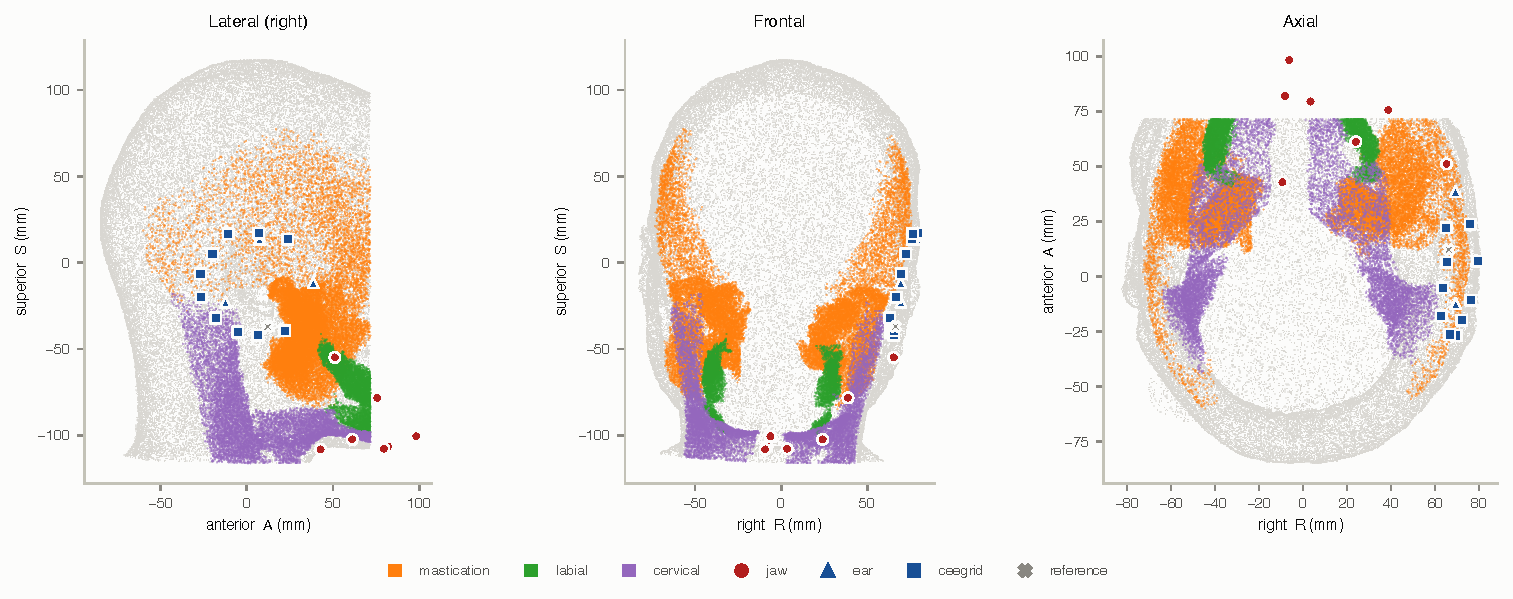
\includegraphics[width=\linewidth,height=0.42\textheight,keepaspectratio]{fig1_head_model.pdf}
\caption{MIDA head model with the ten segmented articulator compartments highlighted, and all 22 electrode positions shown in lateral, frontal and axial views. The face is removed anterior of the eyes at all heights, in accordance with MIDA licence clause 2.3.3.}
\end{figure}


MIDA is commonly cited as containing 153 structures. That figure describes the
CAD/surface distribution. The voxel distribution used here carries \textbf{116
labelled structures}, and every number in this paper derives from the voxel
data. We report 116 and not 153 throughout; the discrepancy is a difference
between two distributions of the same model, not a subsetting choice.

Ten of the eighteen articulator muscles in our target set are individually
segmented and were verified present by label: masseter (66), temporalis /
temporoparietalis (63), medial pterygoid (81), lateral pterygoid (65),
orbicularis oris (75), buccinator (84), mentalis (71), depressor anguli oris
(72), platysma (60), sternocleidomastoid (68).

The suprahyoid and tongue muscles are not individually segmented. Digastric
(both bellies), stylohyoid, mylohyoid, geniohyoid, genioglossus, hyoglossus and
styloglossus are pooled into \texttt{Muscle\ (General)} (label 38; 1,975,307 voxels,
246,872 mm\textsuperscript{3}) and \texttt{Tongue} (label 42; 521,131 voxels, 65,130 mm\textsuperscript{3}). They are
therefore absent from the per-muscle results, which is a limitation of the
source segmentation, not of the method. MIDA also merges temporalis with
temporoparietalis in a single label (63) and carries the temporalis tendon
separately (98); the tendon is excluded, since its conductivity differs from
muscle and it is not a source.

\textbf{Meshing.} The labelled volume was tetrahedralised with SimNIBS 4.6's
\texttt{meshmesh} (Thielscher et al.~2015), using per-label conductivity assignment. The
finite-element electric-field solver this study repurposes for reciprocity is
described in Saturnino et al.~(2019). The base mesh contains
2,140,917 nodes and 15,415,273 elements. SimNIBS meshes the two electrodes into
it at solve time, giving 15,415,668 elements of which 12,294,182 are tetrahedra.

A neck-extended variant was constructed and rejected: it does not conserve
charge, with flux failing to decay toward the domain floor (1.070 mA at S =
\textminus{}182 mm against a 1 mA injection, where the truncated control falls to 0.107 mA
at S = \textminus{}119 mm). Its terminating face is parallel to the base mesh's, displaced
70.001 mm inferiorly along the plane normal against the 70 mm extrusion
requested in \texttt{01c\_extend\_neck.py}. All published results use the truncated mesh;
the consequence for the jaw-versus-ear comparison is quantified in \S{}3.4.

The fitted cut-plane geometry, its agreement with MIDA's own voxel axis, and the mesh-validation checks are given in full in Appendix A.

\subsubsection{2.2 Conductivity assignment}\label{conductivity-assignment}

All conductivities are listed in Table 1 with individual sources and live in a
single file; none is hardcoded elsewhere. All values are quoted at 100 Hz, which
brackets the surface-EMG band.

Air is a numerical choice, not a physical one. True air conductivity is
zero, which makes the FEM system singular, so internal cavities are assigned a
small finite value. The value matters because the stiffness matrix inherits
$\sigma$\_max/$\sigma$\_min as its condition number and SimNIBS solves iteratively. At
$\sigma$\_air = 1 \texttimes{} 10\textsuperscript{\textminus15} S/m the span reaches 1.879 \texttimes{} 10\textsuperscript{15}, the iterative solve does
not converge, and the returned fields are 10--20\texttimes{} too large while a result file
is still written. We use $\sigma$\_air = 1 \texttimes{} 10\textsuperscript{\textminus6} S/m throughout, giving a span of
1.879 \texttimes{} 10\textsuperscript{6}. A pre-flight gate refuses any assignment whose span exceeds
1 \texttimes{} 10\textsuperscript{8}.

The measured insensitivity of every reported gap to that choice is given in Appendix A.

\subsubsection{2.3 Electrode placement}\label{electrode-placement}

All 22 positions are derived from labelled anatomy and snapped to the outer skin
surface, not hand-picked. An interactive picker was rejected because clicked
coordinates cannot be regenerated from a clean checkout, reviewed in a diff, or
defended in Methods.

Each site is defined by an anatomical anchor plus an offset in RAS millimetres,
then projected to the nearest outer-skin voxel along the surface normal.

The target-localisation rule, the derived anatomical midline, and per-site depths are specified in Appendix A.

\texttt{pre\_tragus} is placed 14 mm anterior to the tragus, over the masseter and the
temporomandibular joint, as the retroauricular position with the shortest path
to the mastication group. The ten C-path positions are labelled \texttt{cg01}--\texttt{cg10}
after the cEEGrid layout of Debener et al.~(2015), at 12--18 mm spacing around
the pinna; all 22 sites are shown in Figure 1.

The electrode model is a 10 mm diameter ellipse of 2 mm thickness, matching the
gold cup electrodes of the companion experiment.

\subsubsection{2.4 Reciprocity}\label{reciprocity}

Lead fields are computed by reciprocity, not by forward-solving each source. For
a current dipole at position \textbf{r} with moment \textbf{p} and a recording pair (A,
B), the measured potential difference is

\[V_{AB}(\mathbf{r}, \mathbf{p}) = \mathbf{E}_{\mathrm{recip}}(\mathbf{r}) \cdot \mathbf{p} \, / \, I\]

where \textbf{E}\_recip is the field produced throughout the head by injecting current
\emph{I} between A and B. The lead field for a source at \textbf{r} with unit orientation
\textbf{n} is therefore E\_recip(\textbf{r}) \textperiodcentered{} \textbf{n}.

SimNIBS's tDCS solver computes exactly E\_recip, so it is repurposed here: 1 mA
is injected between each electrode and a common reference (contralateral
earlobe), and the resulting field is read inside every segmented muscle
compartment. The consequence is one solve per electrode instead of one per
source, 22 solves against the order of 10\textsuperscript{5} a forward formulation would require
at MIDA's resolution. The formulations are mathematically equivalent; only cost
differs.

Within each compartment we report the volume-weighted median \textbar E\textbar, which is
robust to the small number of very high-field elements adjacent to compartment
boundaries.

\subsubsection{2.5 Fibre orientation}\label{fibre-orientation}

Muscle is electrically anisotropic and MIDA carries no fibre-direction data, so
orientation is bounded, not assumed.

Deriving fibre directions by principal component analysis on MIDA's own
segmentation is not novel here: it was published by HArtMuT {[}Harmening et al.
2022{]}, which built \textasciitilde3,900 muscle sources from MIDA's labels using that method.
We use the same approach and cite it as precedent.

The isotropic condition is primary: all 22 production solves assign muscle a
single isotropic conductivity of 0.355 S/m. A second, anisotropic condition
assigns a per-element tensor with $\sigma$ = 0.4 S/m along the fibre and 0.1 S/m across
it, aligned to a PCA-derived axis.

PCA is applied only where a principal axis is a meaningful object. It describes
a strap-like muscle; for a sphincter (orbicularis oris), a fan (temporalis), a
sheet (platysma, buccinator) or a multi-layered muscle (masseter, lateral
pterygoid), a single axis is the wrong kind of description, not merely an
imprecise one. Those compartments remain isotropic in both conditions.

The anisotropic condition therefore applies a tensor to 2 of the 10 segmented
muscles. Every other compartment is reported as \textbf{not applied} rather than as
an unchanged or null result, because it was never varied.

The bilateral mirror-symmetry test that gates each axis, and the identical-mesh construction that removes electrode realisation from the anisotropy comparison, are specified in Appendix A.

\paragraph{2.5.1 The anatomically-constrained sweep}\label{the-anatomically-constrained-sweep}

An unconstrained orientation fraction and an anatomically constrained one
answer differently posed questions, because orientation space is not uniformly
reachable. Temporalis demonstrates this: 8.5 \% of the derived fan reverses the
montage preference, close to the unconstrained sweep's 8.0 per cent, but only
the fan's directions are ones the anatomy can realise. Both fractions are taken at the pre-registered cluster
{[}\texttt{results/04q\_table4\_envelope.csv}, \texttt{results/04k\_fan\_fractions.csv}{]}; the same
fan read against all fourteen ear sites gives 0.5 \%, and pairing fractions
across those two bases would compare different comparisons. We therefore sweep
the hemisphere first and intersect with the anatomically permitted set wherever
one can be established, reporting the unconstrained fraction alongside so the
constraint is visible, not implicit. That intersection is available for
temporalis alone; \S{}4.7 states where it is not.

\subsubsection{2.6 Validation}\label{validation}

Validation is layered, and each layer tests something the others cannot.

\textbf{Analytic multilayer sphere.} The full pipeline is run against a four-layer
spherical head model with a closed-form solution. Over 120 source positions
spanning radii 20--75 mm, median RDM is 4.36 \% and median MAG +4.40 \%. This is
the only layer that can detect a uniform scale error, since no invariant
computed on the head mesh can: multiplying every field value by a constant
leaves flux radius-independence, boundary conservation, linearity and
reciprocity symmetry all satisfied. Both figures are reported as validation
results. No pass criterion is stated, because none was fixed before the values
were computed and supplying one now would be a threshold chosen to admit the
numbers it is meant to test.

Three further validation layers (reciprocity verified on the head mesh itself, four physical invariants computed on every solve, a mesh-convergence fit, and two guard meta-tests that protect the validation machinery) are specified in full in Appendix A.

\subsubsection{2.7 Error budget}\label{error-budget}

Every published quantity in this paper is a ratio, one site against another,
ear against jaw, muscle against muscle, and that structure determines how
uncertainty is handled. A term that scales the whole lead field equally cancels
exactly in every ratio and cannot reach a conclusion. A term that varies between
sites survives into all of them. Table 3 is split into two columns on exactly
that distinction, and terms are admitted to the second column only when shown to
vary per site.

The full budget, with per-term magnitudes, is Table 3 in Appendix B.

Four rows are admitted on a second and different basis, and the table marks them
as such. Terms 1, 2, 3 and 7 are known to act on the ratio directionally but are
not quantifiable at current precision, so they carry no value. Admitting them
records that they are unresolved, not absent; it does not claim a
magnitude. The rule above is unchanged, and these rows do not satisfy it.

The distinction is not cosmetic. Electrode contact area would naturally be
treated as a global scale factor; it is not, because each electrode's contact is
realised independently from whatever surface triangles fall beneath it, making
it per-site noise. Conversely a uniform magnitude offset, however large,
subtracts to exactly 0 dB in any site ratio.

\subsubsection{2.8 Reproducibility and pre-registration}\label{reproducibility-and-pre-registration}

Everything is reproducible from a clean checkout given MIDA in \texttt{data/} \textbf{and the mesh that produced these results}; the one
manual step, downloading MIDA, requires registration and is documented in the
repository README. MIDA itself cannot be redistributed under its licence and is
not included.

The mesh-realisation qualification to this claim, and a worked failure case for tables produced without a generating script, are given in Appendix A.

The anatomical prediction was recorded before the model was solved. The
\texttt{expected\_at\_ear} column of the muscle configuration --- predicting strong
retroauricular coupling for temporalis (``directly above ear'') and
sternocleidomastoid (``mastoid attachment'') --- entered the project repository on
2026-08-02. The lead-field results that test that prediction were committed the
following day, 2026-08-03. The prediction therefore precedes the measurement by
a day and by the entire solve pipeline. Both commits are citable by hash in the
public repository; the hashes and the repository link are withheld from this
submission for anonymous review and will be restored in the final version.

\textbf{The prediction was not confirmed, and that is reported here and not removed.}
The first solves appeared to bear it out: temporalis and sternocleidomastoid
both showed a retroauricular advantage, and so did lateral pterygoid, which the
prediction had not named. None survived the orientation and electrode-count
controls (\S{}3.1, \S{}4.8). A pre-registration that is quietly deleted when it fails
records nothing; one that is reported when it fails is doing the work it was
recorded for. It is retained here in its original form, with its outcome stated,
precisely because the model initially appeared to confirm it.

\subsubsection{2.9 Ethics}\label{ethics}

No human subjects were involved. This is a computational modelling study
performed on a licensed anatomical model. No IRB review was required or sought,
and no new imaging, recordings or measurements from living participants were
acquired.

\begin{center}\rule{0.5\linewidth}{0.5pt}\end{center}

\subsection{3. Results}\label{results}

\subsubsection{3.1 Which montage sees which muscle}\label{which-montage-sees-which-muscle}

Reporting one gap per muscle presumes a fibre direction the model does not
contain, and comparing the best of fourteen retroauricular sites against the
best of four jaw sites rewards electrode count, not placement. Both are
controlled. Source orientation is swept over the hemisphere at 200 directions
with the same orientation applied at both electrodes, since only a common
orientation corresponds to a physical source. Electrode count is matched by
drawing four of the fourteen ear sites at random, taking the best, and
repeating; the resulting interval says whether a preference is a property of
the montage or of which sites happen to be available.

The jaw's dominance over the labial group is robust on both axes.
Orbicularis oris, buccinator, mentalis, depressor anguli oris and platysma
favour the jaw at all 200 sampled orientations and at every electrode
subsample. No fibre direction and no four-site selection exists at which a
retroauricular electrode competes for these muscles. The full muscle-by-site
sensitivity matrix is given in Figure 2, and the per-muscle verdicts in
Figure 3.


\begin{figure}[htbp]
\centering
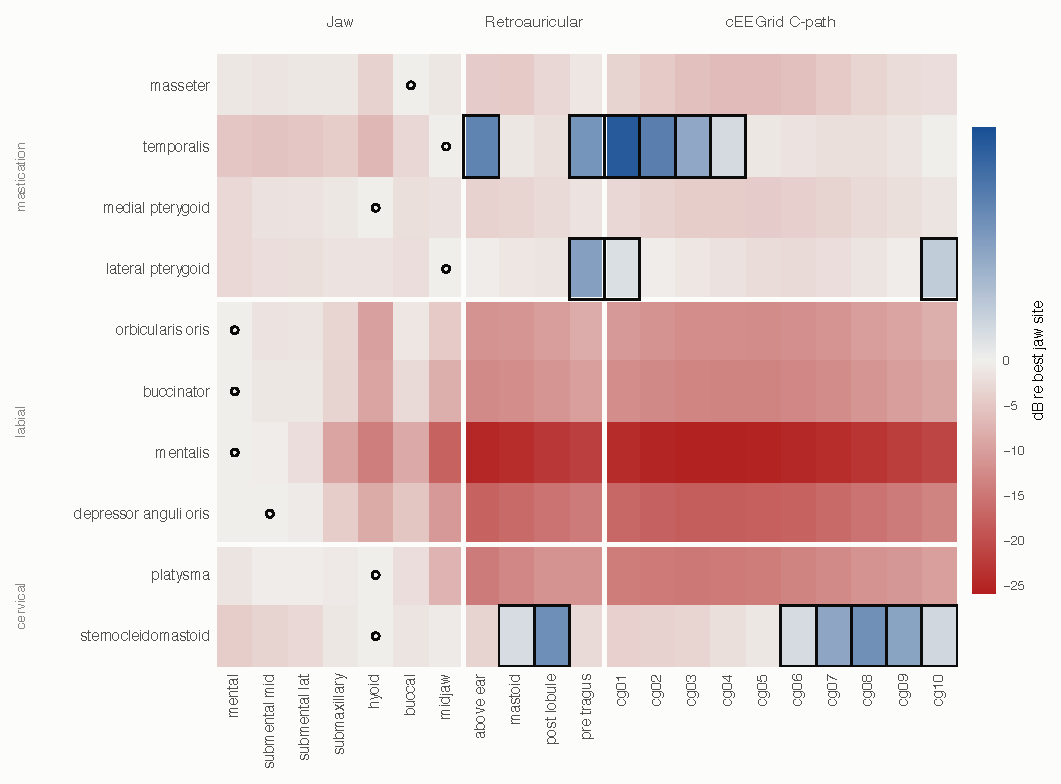
\includegraphics[width=\linewidth,height=0.42\textheight,keepaspectratio]{fig2_sensitivity_matrix.pdf}
\caption{Articulator sensitivity matrix. Median lead field in each segmented muscle compartment for each electrode site, in dB relative to that muscle's best jaw site (0 dB, ringed). Isotropic condition, truncated mesh, 22 electrodes \texttimes{} 10 muscles. The colour scale is diverging about 0 dB: red is attenuation relative to the best jaw site, blue is a site that exceeds it, and boxed cells mark every (site, muscle) pair where a retroauricular electrode beats every jaw electrode. The two arms are not equally scaled (\textminus{}28 to 0 dB against 0 to +4 dB), so colour saturation is not comparable across the midpoint; the boxes carry the sign independently of colour. The 0 dB reference here includes all jaw sites, whereas Figure 3 and Table 4 exclude those within 10 mm of the truncation face, so the named best jaw site differs for some muscles.}
\end{figure}



\begin{figure}[htbp]
\centering
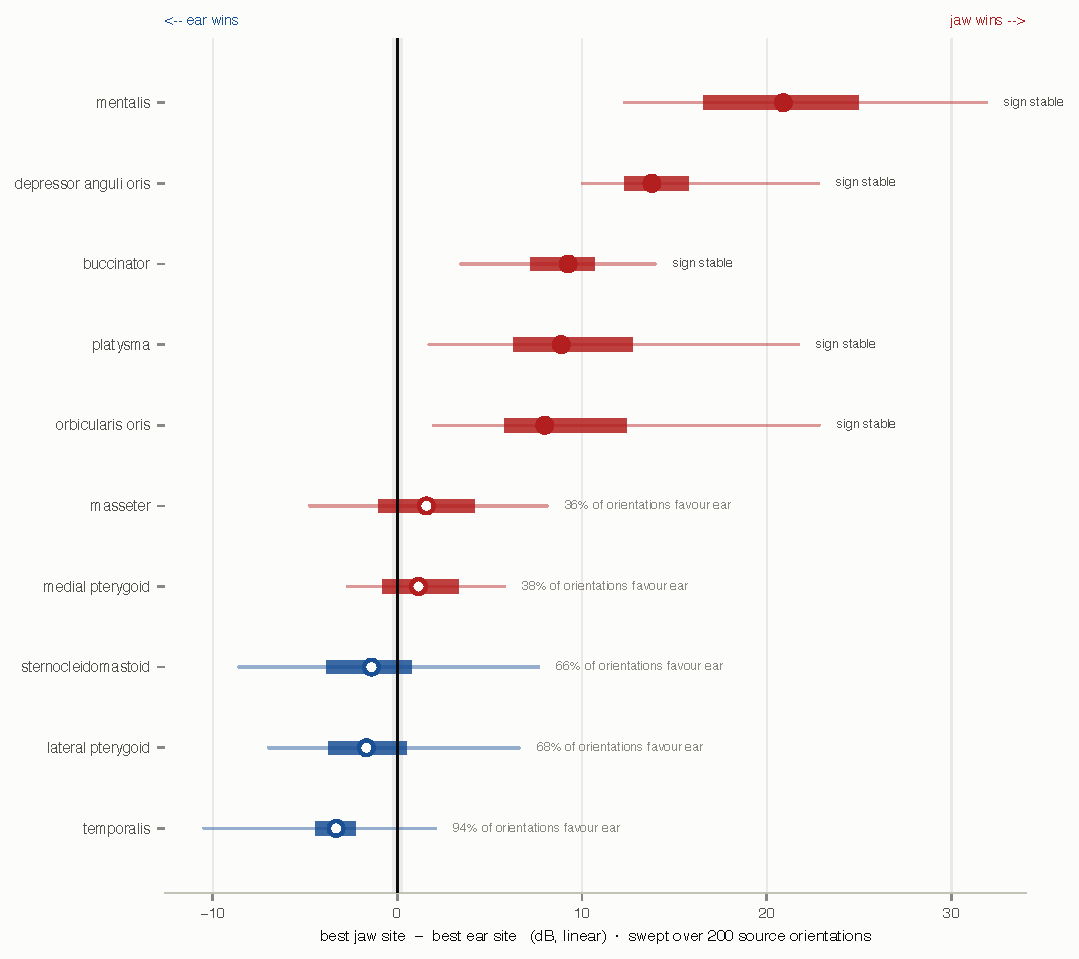
\includegraphics[width=\linewidth,height=0.42\textheight,keepaspectratio]{fig3_complementarity_map.pdf}
\caption{Which montage sees which muscle. For each articulator, the difference between the best jaw site and the best retroauricular site, in dB. Negative bars are muscles the ear sees more strongly. Jaw sites within 10 mm of the truncation face are excluded. The shaded band is the measured electrode-meshing floor (0.27 dB, with the lighter band extending to its 95 \% CI upper bound of 0.65 dB). The axis is linear in dB and not a rank, because the asymmetry between the arms is itself a result: the jaw's advantages reach +20.90 dB while the ear's reach only \textminus{}3.31 dB. Both numbers are emitted from the figure's own source file by src/04m\_caption\_numbers.py, which fails the build if a caption and its figure disagree.}
\end{figure}


No articulator favours the ear on both axes. Temporalis is the closest,
and it does not clear the bar. Over the fibre field derived from the anatomy
(\S{}2.5.1) it reaches \textminus{}1.147 dB at the pre-registered four-site cluster, with
91.5 per cent of fibre directions agreeing, but its matched-count interval is
\textbf{{[}\textminus{}1.453, +5.458{]}} and only \textbf{50.5 per cent} of the four-site
retroauricular subsets favour the ear at all. Whether the ear wins for
temporalis is decided by which four electrodes a device happens to carry, not
by the anatomy.

The two treatments disagree, and the anatomy-specific one governs. Under a
uniform orientation sweep temporalis reaches \textminus{}2.571 dB with 92.0 per cent of
orientations agreeing and an interval of {[}\textminus{}3.308, \textminus{}0.035{]} that excludes zero ---
on that treatment it would be reported as favouring the ear. The sweep assumes
source orientation is uniformly distributed over the sphere, which is the right
default when fibre direction is unknown and the wrong one for a muscle whose
fibres converge on a single identifiable insertion.

The interval is computed exactly, not sampled. Fourteen candidate ear sites
taken four at a time gives 1001 possible subsets, so every one is enumerated and
the interval is a complete description of that set rather than an estimate from
draws. It therefore carries no seed and no sampling error. For the derived fibre
field the enumeration varies electrodes alone, with the fibre orientation held
fixed, so the resulting spread reflects site availability and nothing else.
Temporalis gives a median gap of \textminus{}1.147 dB with an interval of
{[}\textminus{}1.453, +5.458{]} dB, favouring the ear in 50.5 per cent of subsets
{[}\texttt{results/04p\_headline\_interval.csv}{]}.

We report the derived result because it removes an assumption rather than
adding one, and the pre-registered reading (\S{}2.8) committed to that treatment
before the derivation was run. The uniform-sweep figure is reported alongside
it so the dependence is visible: \textbf{this verdict rests on the fibre derivation,
and a reader who rejects that derivation should read temporalis as favouring
the ear by 2.57 dB.}

Two show no preference that survives electrode subsampling.
Sternocleidomastoid (\textminus{}0.973 dB at the cluster, 60.5 per cent of orientations,
interval {[}\textminus{}1.40, +1.27{]}) and lateral pterygoid (\textminus{}1.564 dB, 65.5 per cent,
{[}\textminus{}1.59, +1.09{]}) both have intervals crossing zero. Their apparent advantage
depends on which four sites are available and is not a property of the
montage. Reported at the unmatched argmax over fourteen sites they would read
\textminus{}1.402 and \textminus{}1.679 dB, which is why the matched comparison is the one reported.

Two favour the jaw robustly across sites but not across orientation.
Masseter and medial pterygoid have subsample intervals entirely positive, but
31.5 and 34.5 per cent of sampled orientations reverse them at the published
cluster {[}\texttt{results/04n\_site\_set\_sensitivity.csv}{]}. A single label would discard
one axis or the other, so both are reported (Table 4).

\subsubsection{3.2 Anisotropy changes the field but not the comparison}\label{anisotropy-changes-the-field-but-not-the-comparison}

The isotropy assumption does not measurably affect any site-to-site ratio
(Figure 4).
Applying a fibre tensor changes the jaw-versus-ear gap by \textminus{}0.085 dB for
sternocleidomastoid, \textminus{}0.010 dB for medial pterygoid, +0.137 dB for temporalis
and +0.036 dB for lateral pterygoid. Every one of these lies below the 0.27 dB
measured electrode-meshing floor, including for the two compartments that
carry a tensor. Anisotropy raises the absolute lead field substantially, by
roughly 5 dB in medial pterygoid, but it does so at the jaw and ear sites
alike, so the effect subtracts out of every ratio this paper reports.


\begin{figure}[htbp]
\centering
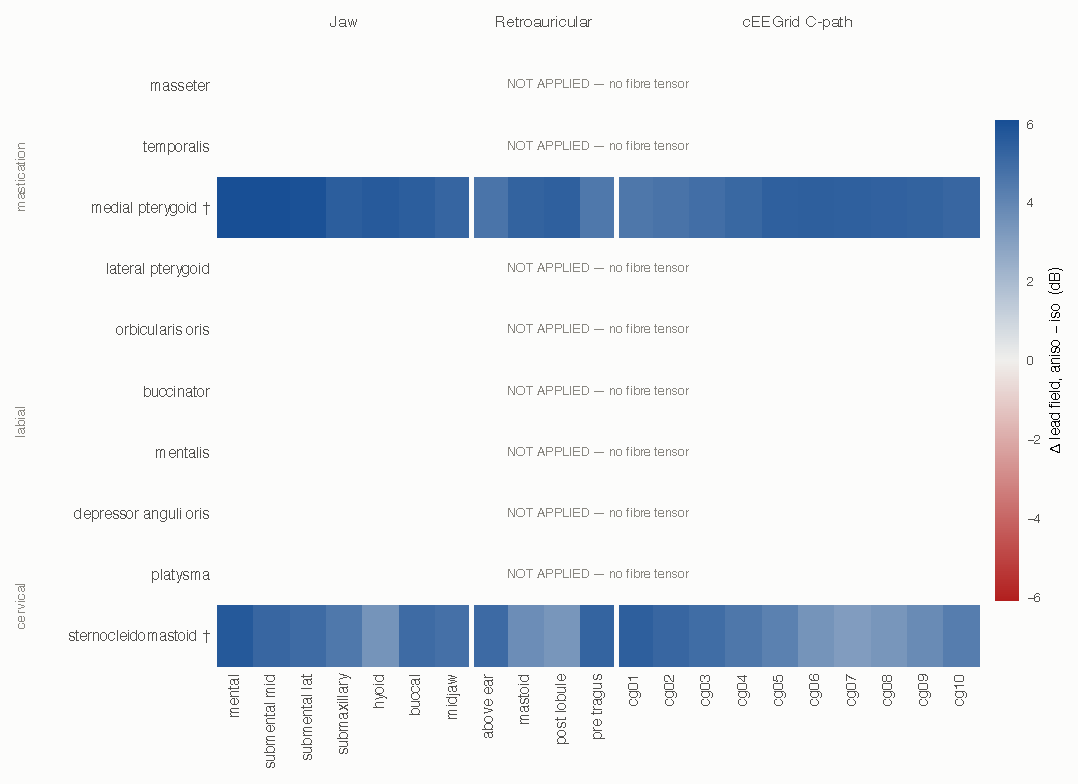
\includegraphics[width=\linewidth,height=0.42\textheight,keepaspectratio]{fig4_anisotropy_delta.pdf}
\caption{Anisotropy robustness check. Change in lead field between the isotropic and anisotropic conditions, 20\textperiodcentered{}log\textsubscript{1}\textsubscript{0}(aniso/iso), per cell. The anisotropic condition is solved on the isotropic run's own mesh, so the two differ in conductivity alone and carry no electrode-realisation noise. A fibre tensor is applied to 2 of 10 muscles, sternocleidomastoid and medial pterygoid. Rows without a tensor are labelled not applied, not zero: they were never varied, so no null result was measured for them.}
\end{figure}


The null carries a bound; it is not an absence of evidence, and it has a
practical consequence: for coupling \emph{ratios} between electrode sites, a
muscle-fibre tensor is not worth the modelling effort in a head model of this
resolution. Absolute lead-field values are a different matter and are affected.

\subsubsection{3.3 The tissue-conductivity contrast is a small term with a muscle-dependent sign}\label{the-tissue-conductivity-contrast-is-a-small-term-with-a-muscle-dependent-sign}

Solving the full montage twice on identical geometry, once with adipose at
0.025 S/m and once with both adipose compartments set to muscle conductivity,
attributes any difference to material properties alone, since source-to-electrode
distance is unchanged by construction. The second condition is a counterfactual
used to decompose mechanism; the gaps reported throughout this paper are the
first, because real anatomy contains adipose tissue.

This section decomposes the \textbf{jaw montage's advantage}. An earlier version
decomposed a retroauricular deficit, which no longer exists as a result: no
articulator resolves in the ear's favour (\S{}3.1), so there is no ear advantage
whose mechanism needs explaining. What remains to be explained is why the jaw
montage wins, and by how much of that the tissue contrast is responsible.

The contribution is not uniform in sign across muscles, because which electrode
is best differs by muscle and the shift is not uniform within a montage:

{\def\LTcaptype{none} % do not increment counter
\begin{longtable}[]{@{}
  >{\raggedright\arraybackslash}p{\dimexpr(\linewidth - 10\tabcolsep)*2200/10000\relax}
  >{\raggedright\arraybackslash}p{\dimexpr(\linewidth - 10\tabcolsep)*1600/10000\relax}
  >{\raggedright\arraybackslash}p{\dimexpr(\linewidth - 10\tabcolsep)*1800/10000\relax}
  >{\raggedright\arraybackslash}p{\dimexpr(\linewidth - 10\tabcolsep)*1400/10000\relax}
  >{\raggedright\arraybackslash}p{\dimexpr(\linewidth - 10\tabcolsep)*3000/10000\relax}@{}}
\toprule\noalign{}
Muscle & As modelled & Without contrast & Change & Contrast's role \\
\midrule\noalign{}
\endhead
\bottomrule\noalign{}
\endlastfoot
temporalis & \textminus{}3.801 & \textminus{}4.923 & \textminus{}1.121 & suppresses 29.5 \% \\
sternocleidomastoid & \textminus{}1.958 & \textminus{}1.547 & 0.411 & contributes 21.0 \% \\
lateral pterygoid & \textminus{}1.855 & \textminus{}1.532 & 0.323 & contributes 17.4 \% \\
medial pterygoid & 1.147 & 1.245 & 0.098 & suppresses 8.6 \% \\
masseter & 1.700 & 1.668 & \textminus{}0.032 & contributes 1.9 \% \\
orbicularis oris & 8.192 & 9.286 & 1.093 & suppresses 13.3 \% \\
platysma & 8.844 & 8.901 & 0.057 & suppresses 0.6 \% \\
buccinator & 10.033 & 9.848 & \textminus{}0.185 & contributes 1.8 \% \\
depressor anguli oris & 14.607 & 14.001 & \textminus{}0.606 & contributes 4.1 \% \\
mentalis & 21.945 & 19.082 & \textminus{}2.863 & contributes 13.0 \% \\
\end{longtable}
}

For the labial group, where the jaw's advantage is largest, the contrast
accounts for a small and inconsistent fraction of it, and not in one direction:
the contrast \emph{builds} 2.86 dB of the mentalis gap while \emph{suppressing} 1.09 dB of
the orbicularis oris gap. For the four muscles
whose gaps sit closest to zero, the contrast is of the same order as the gap
itself, which is part of why those gaps do not resolve.

The mechanism is therefore geometric, not material. Removing the
single largest conductivity contrast in the intervening tissue leaves every
montage assignment unchanged and moves no gap across zero. This is consistent
with \S{}3.5, where collapsing all non-muscle soft tissue to one conductivity also
preserves every assignment while moving magnitudes.

\subsubsection{3.4 Truncation sensitivity}\label{truncation-sensitivity}

The inferior truncation lies closer to the jaw montage than to the
retroauricular montage, so the cut plane could in principle inflate the jaw
side. Perpendicular clearance to the fitted plane places 2 jaw sites within
10 mm of it (\texttt{hyoid} 7.76 mm and \texttt{submental\_lat} 9.76 mm); the next nearest is
\texttt{submental\_mid} at 10.76 mm. The closest ear site, \texttt{cg09}, is 75.27 mm away.

Removing the near-cut sites moves the median gap from +4.68 dB to +4.52 dB, a
shift of \textminus{}0.17 dB. No muscle changes sign (0 of 10). The largest individual
movements are \texttt{medial\_pterygoid} \textminus{}0.88, \texttt{sternocleidomastoid} \textminus{}0.54 and
\texttt{platysma} \textminus{}0.37 dB. The reported advantage is not an artefact of proximity to
the truncation. The sensitivity reported here measures the effect of excluding
the most exposed sites. It does not bound the residual boundary artefact on the
sites that remain, which is addressed in \S{}4.7.

The 10 mm grouping above is descriptive. The reported subsets span every
admissible site set for any near-cut threshold between 9.757 mm and 15.264 mm, a
window of 5.507 mm, so no conclusion here depends on where in that range the
threshold is placed.

For the muscles that do not move, the best jaw electrode was never a near-cut
site, so excluding them cannot change the maximum: those muscles are immune by
construction rather than by luck.

\begin{center}\rule{0.5\linewidth}{0.5pt}\end{center}

\subsubsection{3.5 A homogeneous conductor reaches the same verdicts}\label{a-homogeneous-conductor-reaches-the-same-verdicts}

A homogeneous soft-tissue conductor reproduces every montage assignment.
Setting skin, adipose and the non-muscle soft tissues to a single conductivity,
with geometry, electrodes and sources held exactly fixed, changes no muscle's
montage preference. Eight of ten gap magnitudes move by more than the 0.27 dB
floor, with a median shift of 0.482 dB and a maximum of 3.271 dB (mentalis).

The direction is not uniform. Temporalis's retroauricular advantage \emph{grows}
under the homogeneous conductor, from \textminus{}2.571 to \textminus{}3.724 dB at the pre-registered
cluster {[}\texttt{results/04r\_homog\_cluster.csv}{]}, so the anatomically resolved model
reports that result more conservatively than a simpler one would.
Sternocleidomastoid and lateral pterygoid move the other way.

This locates what the detailed conductor is required for. The question of
which montage sees which muscle is answerable without it. The question of by
how much is not, and a design table quoting decibels needs it.

\subsubsection{3.6 Placement by anatomical target outperforms density}\label{placement-by-anatomical-target-outperforms-density}

Placement chosen by anatomical target outperforms arbitrary placement. The
four-site retroauricular cluster, above the ear, over the mastoid, behind and
below the lobule, and anterior to the tragus, was specified by anatomical
target in the project repository before any solve was run. Compared against
the median of random four-site draws from the same fourteen candidates, it is
1.07 dB better for lateral pterygoid (\textminus{}1.564 against \textminus{}0.498) and equivalent
for sternocleidomastoid (\textminus{}0.973 against \textminus{}0.979)
{[}\texttt{results/04h\_matched\_counts.csv}{]}.

Neither of the two sites that won the unmatched argmax for temporalis and
sternocleidomastoid is in that cluster, which is the same point from the other
direction: an argmax over fourteen densely spaced positions rewards density,
while a four-site montage rewards placement. For a device constrained to a
small number of contacts, where they go matters more than how many candidates
were considered.

\subsection{4. Discussion}\label{discussion}

\subsubsection{4.1 The montages are not complementary}\label{the-montages-are-not-complementary}

An earlier framing of this work treated jaw and retroauricular montages as
complementary, each better for some articulators, and that framing does not
survive its own controls. Every articulator this model can resolve favours the
jaw montage. The three that appeared to favour the ear, all of them attaching at
or near the temporal bone, are the three whose gaps come closest to zero, but
none crosses it once source orientation and electrode count are controlled
(\S{}3.1, \S{}4.8).

The result is therefore one-sided, not a trade. A retroauricular montage
is not a repositioning of the jaw montage that exchanges one muscle group for
another; it is a montage that loses the labial group by 8.11 to 22.40 dB and
returns nothing measurable. Anatomical proximity to a bony attachment does
predict which retroauricular sites are competitive, and in the right order, but
competitive is not the same as better.

Temporalis is the clearest case and the one that took longest to settle, and it
is the one place where this conclusion depends on a modelling choice, not on a
control. Under a uniform orientation sweep it favours the ear by 2.57 dB with an
interval excluding zero. Under the fibre field derived from the label volume it
favours the ear by 1.147 dB with an interval of {[}\textminus{}1.453, +5.458{]}, and does not
resolve. The difference is not a correction of an error; it is the difference
between assuming source orientation is uniform over the sphere and deriving it
from where the muscle actually attaches. That difference also changes what the
accompanying intervals measure. Under the uniform sweep, orientation is a
sampled dimension and the interval averages over 200 directions within each
draw; under the derived field there is no orientation dimension to average over,
and the interval reflects site selection alone. The two intervals answer
different questions and should not be read as one quantity under two fibre
models. We take the derived field because it removes an assumption, and we state
the dependence rather than burying it: \textbf{the claim that no articulator favours
the retroauricular montage rests on the temporalis fibre derivation, and is the
single most attackable point in this paper.} \S{}4.6 makes it falsifiable.

\subsubsection{4.2 An anatomical prediction that did not survive}\label{an-anatomical-prediction-that-did-not-survive}

The prediction recorded before solving (\S{}2.8) was that muscles attaching at or
near the temporal bone would couple preferentially to retroauricular sites.
The anatomy behind it is not in dispute: temporalis originates in the temporal
fossa directly beneath the superior cEEGrid row, sternocleidomastoid inserts on
the mastoid process, and lateral pterygoid inserts at the mandibular condyle,
which articulates with the temporal bone's mandibular fossa.

The uncontrolled comparison reproduced it exactly, those three muscles, and only
those three, showed a retroauricular advantage, each at the site the anatomy
implied. Under matched electrode counts and a derived and not an assumed fibre
field, none of the three survives (\S{}3.1).

The prediction is therefore reported as a \textbf{failed} one, and its failure is
informative in a way its confirmation would not have been. Proximity to a bony
attachment predicts which sites are \emph{competitive}, the three near-temporal
muscles are the three whose gaps come closest to zero, and the ordering is
correct, but it does not predict that any of them crosses. A volume conductor is
not a proximity argument: the current returns through whatever path the
conductivities allow, and an attachment adjacent to an electrode does not make
that electrode the better observer of the fibre.

\subsubsection{4.3 The mechanism is distance, not intervening tissue}\label{the-mechanism-is-distance-not-intervening-tissue}

For the labial group the ear's deficit is predominantly geometric, though the
material contribution varies widely within the group: the adipose--muscle
conductivity contrast accounts for 0.6 per cent of the gap for platysma and
13.3 per cent for orbicularis oris. The remainder in every case is
source-to-electrode distance, and the attenuation-against-depth relation that
produces it is shown in Figure 5. The share is largest where the gap is
smallest, and that is mostly a denominator effect rather than a difference in
the tissue's role. The absolute contribution of the contrast is of comparable
size across muscles, 0.03 to 2.86 dB, while the gaps it is measured against
span an order of magnitude. Expressed as a share it therefore reaches 21 per
cent for the three muscles whose gaps come closest to zero and falls to 0.6
per cent for the labial group, where the jaw's advantage is largest. Neither
figure describes a different mechanism; they describe the same term divided by
different quantities.


\begin{figure}[htbp]
\centering
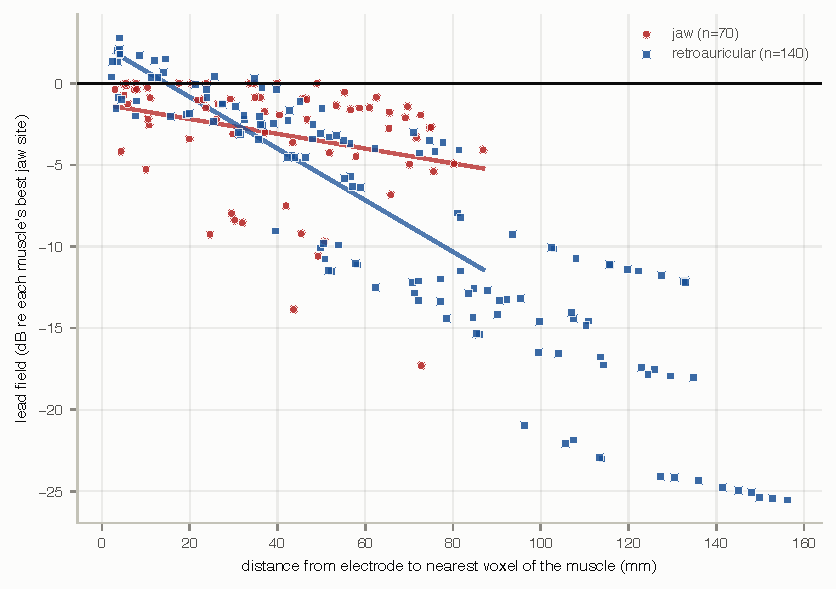
\includegraphics[width=\linewidth,height=0.42\textheight,keepaspectratio]{fig5_attenuation_vs_distance.pdf}
\caption{Attenuation against source-electrode distance. One point per (electrode, muscle) pair: straight-line distance from the electrode to the nearest voxel of that muscle compartment against the lead field in dB relative to that muscle's best jaw site, isotropic condition, truncated mesh. The two montages do not lie on the same attenuation curve. Fitted over the 3 to 87 mm range where both montages have electrodes, the retroauricular sites fall off at \textminus{}0.158 dB/mm against the jaw's \textminus{}0.045 dB/mm, a factor of 3.5 [results/04s\_fig3\_slopes.csv]. A retroauricular electrode therefore loses signal with distance more than three times as fast as a jaw electrode does, which is the geometric mechanism behind the labial-group deficit reported in \S{}4.3. Lines are least-squares fits over the overlapping range only, so the comparison is made where both montages have data, not extrapolated across the ear's longer reach.}
\end{figure}


Limb studies cannot make this separation, because adding a fat layer changes
material properties and source-to-electrode distance together (Kuiken et al.
2003). A labelled head model can, because conductivity is changed with geometry
held exactly fixed. The limb geometry cannot support that comparison at all, and
here it costs one additional solve.

The material share is not a dose response. Across the muscles for which a layer
profile exists, it correlates \emph{negatively} with the adipose fraction of the
muscle-to-skin path (Spearman $\rho$ = \textminus{}0.955, p = 0.001, n = 7): platysma sits at
0.650 fat fraction and 0.6 per cent material share, while sternocleidomastoid
sits at 0.225 and 21 per cent. At n = 7 a single muscle could carry that
relationship, so it was tested: dropping each muscle in turn leaves $\rho$ between
\textminus{}0.928 and \textminus{}0.986 and p below 0.01 in all seven cases
{[}\texttt{results/04t\_correlation\_robustness.csv}{]}; the seven muscles and that
relationship are plotted in Figure 6. The strength of that relationship shows
the swap is measuring adipose path and not something incidental, but its sign
shows it does so through cancellation. The reported share is \textbar $\Delta$gap\textbar{} / \textbar gap\textbar, and
a muscle embedded uniformly in fat has both the jaw and the ear route shifted
together, so the change subtracts out of the ratio. The quantity that would
track positively is the \emph{difference} between how the two routes traverse fat,
which this study does not form. The same cancellation makes a uniform magnitude
offset invisible in every ratio reported here; it turned up here where we had
not expected it.


\begin{figure}[htbp]
\centering
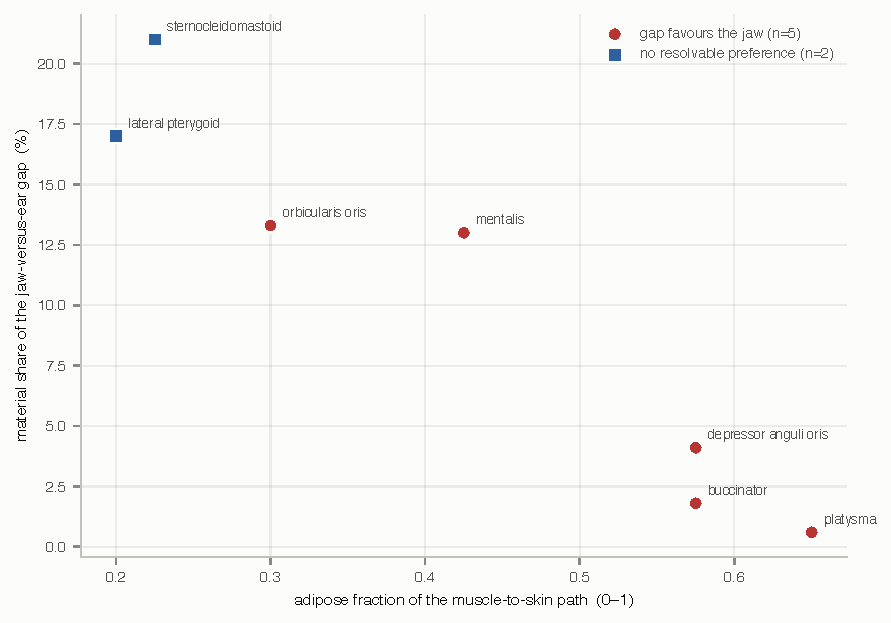
\includegraphics[width=\linewidth,height=0.42\textheight,keepaspectratio]{fig6_material_share_vs_fat.pdf}
\caption{Material share falls as the adipose path grows. For each of the seven muscles with a layer profile, the adipose fraction of the muscle-to-skin path against the material share of that muscle's jaw-versus-ear gap. The relationship is negative (Spearman rho = -0.955, p = 0.001, n = 7): more fat on the path means a \emph{smaller} material share, not a larger one, because a muscle embedded uniformly in fat has both the jaw and the ear route shifted together and the change cancels in the ratio. Leave-one-out leaves rho between -0.928 and -0.986 with p below 0.01 in every case, so no single muscle carries it. Points are marked by whether the muscle's gap resolves to the jaw or reaches no resolvable preference. No trend line is drawn: these are seven independent muscles, not a series, and Spearman is a rank statistic that claims no functional form.}
\end{figure}


Applied to the three muscles whose gaps come closest to zero, temporalis,
sternocleidomastoid and lateral pterygoid, the same decomposition returns a
modest term whose sign varies between them.

For temporalis the contrast acts against the gap, not for it: removing it
would enlarge the gap from \textminus{}3.801 to \textminus{}4.923 dB. The direction is worth stating
because it is the opposite of the intuitive reading, the tissue contrast is not
what produces temporalis's proximity to zero; it is part of what holds it there.
It does not change the verdict, which is set by the matched\textminus{}count interval and
not by this term. For sternocleidomastoid and lateral pterygoid the contrast acts
with the gap, supplying 21.0 and 17.4 per cent of it respectively.

Across all ten muscles the decomposition has the same shape, drawn in Figure 7: a
geometric term that sets the size of the gap and a material term that trims it.
The material term never exceeds 2.9 dB in magnitude, against geometric terms
reaching 19.1 dB, and it changes sign. It moves five muscles toward the jaw and
five toward the ear. That sign change is the reason no single material share is
quoted for the set, and the reason the shares above are reported muscle by
muscle.


\begin{figure}[htbp]
\centering
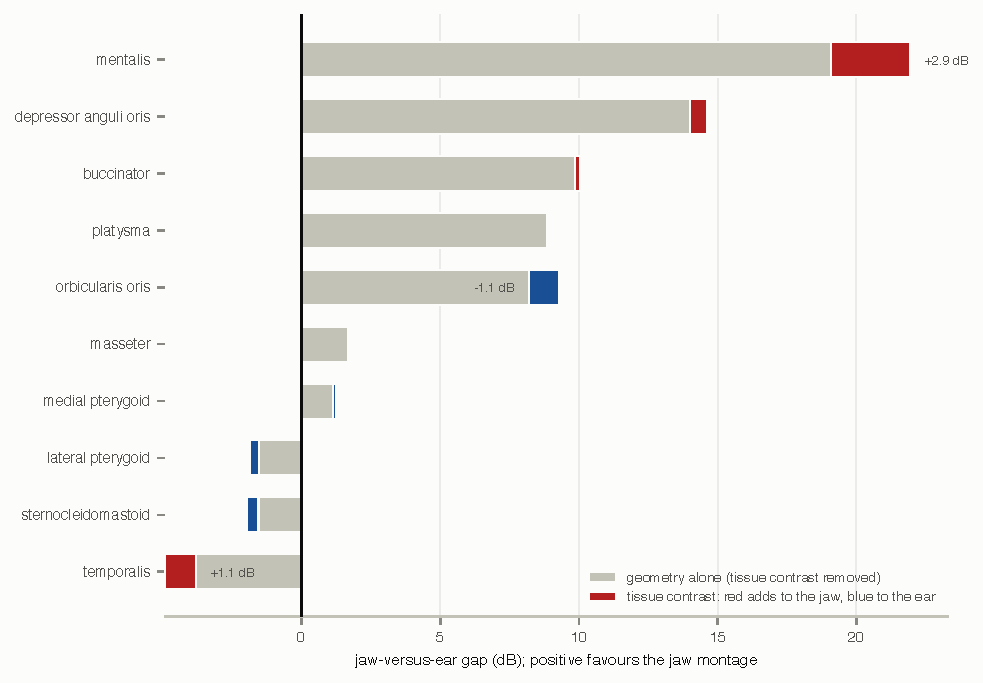
\includegraphics[width=\linewidth,height=0.42\textheight,keepaspectratio]{fig7_gap_decomposition.pdf}
\caption{Geometry sets the gap, tissue only trims it. Each muscle's jaw-versus-ear gap split into the part that survives when the adipose-muscle conductivity contrast is removed, with geometry held exactly fixed, and the part that does not. Positive is a jaw advantage. The geometric term reaches 19.1 dB; the material term never exceeds 2.9 dB and changes sign, moving five muscles toward the jaw and five toward the ear. A single material share for the set would average that sign change away, which is why the text reports shares muscle by muscle.}
\end{figure}


Figure 8 puts the mechanism on the anatomy itself. Taking one representative
electrode from each montage, mental for the jaw and mastoid for the ear, and
mapping the ratio of their two sensitivity fields on a plane that contains both
electrodes and the orbicularis oris centroid, the head separates into a jaw
territory and an ear territory with a crossover running between them.
Orbicularis oris sits 45 mm from the jaw electrode and 141 mm from the ear
electrode, and the jaw is 13.5 dB louder there; temporalis sits on the far side
of the crossover, 116 mm from the ear electrode against 155 mm from the jaw, and
the ear is 4.4 dB louder. The second panel shows the two electrodes falling on
one decay curve, not two. Pooled over the twenty compartment-and-electrode
pairs, log \textbar E\textbar{} against log distance gives Spearman rho = -0.961 (p = 2e-11) with
a slope of -1.42. For nine of the ten muscles the closer electrode is the louder
one; the exception is masseter, where the ear electrode is nearer by 1.9 mm and
the jaw is nonetheless 4.1 dB louder, and it is the only muscle in the set whose
ordering is decided by something other than distance. The figure plots \textbar E\textbar{} for
single electrodes, not the projected lead field for the full montages, so it
carries the mechanism and not the verdicts, which remain those of Table 4.


\begin{figure}[htbp]
\centering
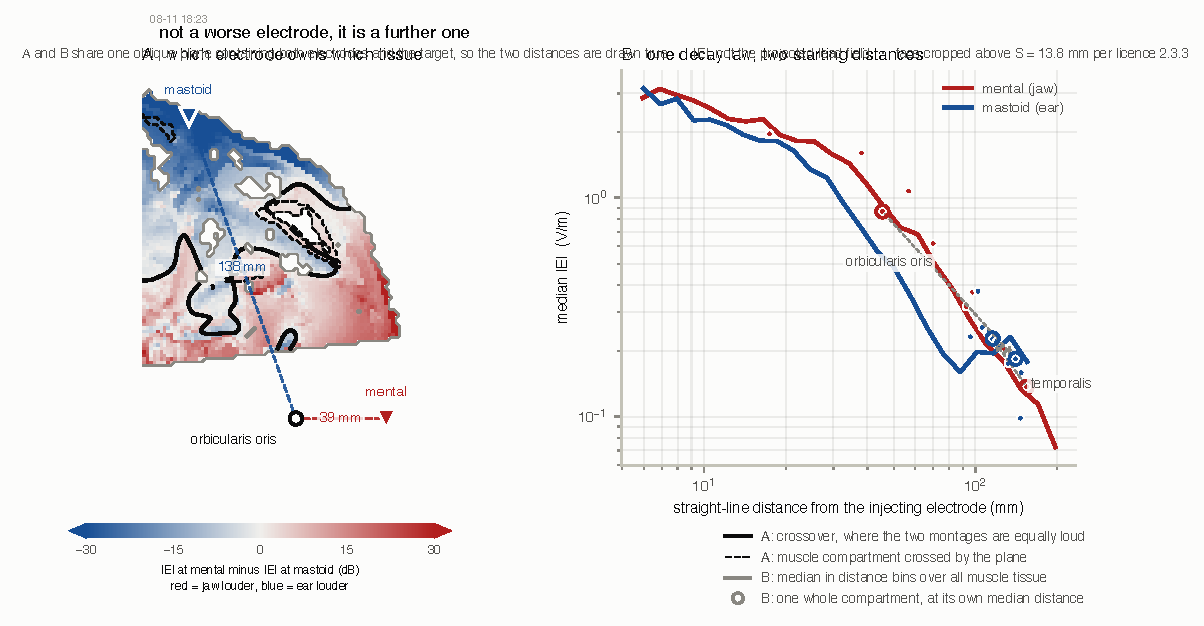
\includegraphics[width=\linewidth,height=0.42\textheight,keepaspectratio]{fig8_distance_mechanism.pdf}
\caption{The gap follows distance. \emph{Left:} the ratio of two sensitivity fields, one from a jaw electrode (mental) and one from a retroauricular electrode (mastoid), on a plane containing both electrodes and the orbicularis oris centroid, so the two distances are drawn true, not projected. Red is a jaw advantage, blue an ear advantage, and the heavy line is the crossover where the two are equally sensitive. \emph{Right:} median |E| against straight-line distance from the injecting electrode, in distance bins over all muscle tissue, with each segmented compartment marked at its own median distance. The two electrodes lie on one decay curve, not two: pooled over the twenty compartment-and-electrode pairs, log |E| against log distance gives Spearman rho = -0.961 (p = 2e-11), slope -1.42. For nine of ten muscles the closer electrode is the louder one; masseter is the exception. |E| is the field magnitude for a single electrode, the upper bound over source orientations, not the projected lead field for a montage, so this figure carries the mechanism and not the verdicts. The plane is cropped above the orbital rim under MIDA licence clause 2.3.3.}
\end{figure}


\subsubsection{4.4 What this licenses for device design}\label{what-this-licenses-for-device-design}

The design statement this supports is a negative one with a number attached. A
retroauricular montage loses the labial group by 8.1 to 22.4 dB, and buys
nothing reliable in return. No articulator in this study favours the
retroauricular montage once source orientation and electrode count are
controlled.

That is more useful to a device team than a small positive margin would have
been. An ear-worn form factor is chosen for wearability, not for signal, and the
question a designer needs answered is what it costs. The answer is that it costs
most of the anterior articulators outright and returns nothing measurable, not
that it trades one muscle group for another.

Three apparent advantages did not survive. Temporalis, sternocleidomastoid and
lateral pterygoid each showed a retroauricular advantage at the unmatched
comparison, and each dissolved: their gaps depend on which four electrodes a
device carries, not on the anatomy (\S{}3.1). A device built around any of them
would be built on a site-selection lottery. Anyone reading a retroauricular
advantage off a model that does not match electrode counts between montages
should expect the same.

What does transfer is that placement method matters more than the marginal
advantages did. A four-site cluster chosen by anatomical target outperforms an
arbitrary four-site draw from the same candidates (\S{}3.6). For a device
constrained to a few contacts, where they go is the lever that remains.

\textbf{This study does not identify an optimal montage, and the reason is the control
that produced its main result.} Selecting the best four of the twenty-one modelled positions that belong to a montage is an argmax over densely spaced candidates, which is the
operation \S{}4.8 shows to be untrustworthy: ten of the fourteen retroauricular
positions lie on a cEEGrid path at 12 to 18 mm spacing, so a search across them
rewards how many were solved. That objection applies to any montage this study
could name, so it names none.

What can be reported without such a search is the strongest single site for each
articulator, with its margin to the runner-up, given as Table 5. The margins are
small, 0.03 to 1.02 dB, and four of the ten sit at or below the 0.65 dB upper
bound of the meshing floor's 95 \% CI, so for mentalis, depressor anguli oris,
platysma and sternocleidomastoid this model does not resolve which single
electrode is best. No muscle's runner-up sits in the other montage, though: all
ten second-best sites share a montage with their best. The site-level argmax is
fragile and the montage-level assignment is not, which is the assumption every
comparison in this paper rests on and which had not been tested on its own.

The strongest site is a jaw site for seven of the ten articulators. The three
served best by a retroauricular site, temporalis, lateral pterygoid and
sternocleidomastoid, are the three whose montage-level advantages do not survive
the controls (\S{}4.8). Both statements hold together: an ear site can be the
strongest single electrode for a muscle while a four-site ear montage still
fails to beat a four-site jaw montage on that same muscle.

A montage recommendation would need two things this study does not supply.
Coupling strength is not decoding accuracy, and two sites coupling strongly to
one muscle carry less joint information than their individual couplings suggest;
what a decoder consumes is channel independence. It would also need the
articulators this model cannot separate, since the tongue and suprahyoid
compartments are pooled in MIDA (\S{}4.7) and carry a large share of articulation,
so no placement statement derived here covers them.

\subsubsection{4.5 Contamination, described muscle by muscle}\label{contamination-described-muscle-by-muscle}

The EEG literature has documented mastoid and retroauricular electromyographic
contamination for decades as a nuisance to be suppressed {[}Goncharova et al.
2003; Yao et al.~2019{]}. This model says what that contamination consists of. The
three compartments a retroauricular electrode couples to most strongly, relative
to the canonical jaw montage (Figure 2), are temporalis, sternocleidomastoid
and lateral pterygoid, and their best positions differ, so contamination at
\texttt{cg01} is not the same mixture as contamination at \texttt{cg08}. The pooled
suprahyoid compartment contributes to that mixture as well; its field under
the retroauricular montage is shown in Figure 9.


\begin{figure}[htbp]
\centering
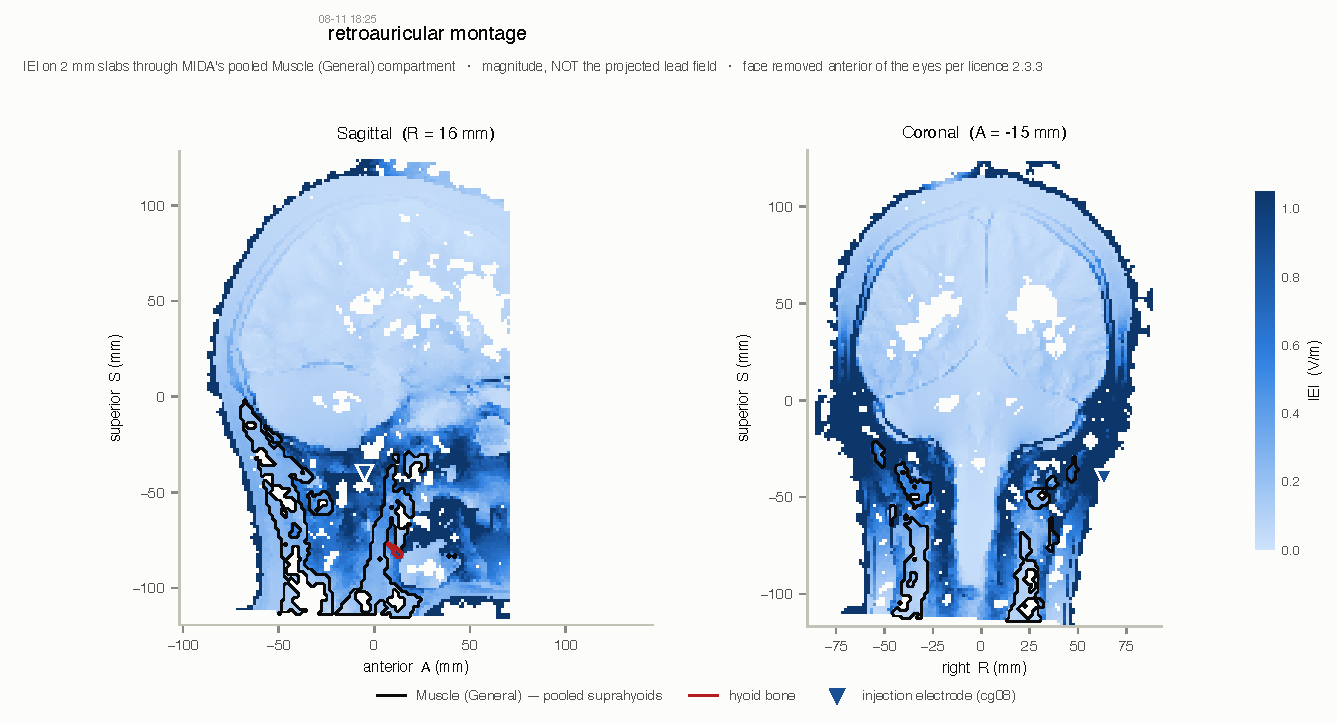
\includegraphics[width=\linewidth,height=0.42\textheight,keepaspectratio]{fig9_suprahyoid_field.pdf}
\caption{Suprahyoid sensitivity field. Sagittal and coronal slices of |E| through the pooled Muscle (General) compartment for the retroauricular montage, with the mastoid notch, hyoid greater horn and the corridor between them overlaid. Reported as a field and not as per-muscle values because MIDA does not segment the suprahyoid group.}
\end{figure}


That is usable in the rejection direction as well as the sensing one. A spatial
filter informed by which muscle dominates at which contact is a different object
from one treating retroauricular electromyography as a single nuisance
component.

\subsubsection{4.6 A specific prediction for a companion experiment}\label{a-specific-prediction-for-a-companion-experiment}

This model makes a falsifiable prediction for a physical experiment recording
both montages simultaneously, and the prediction is a null.

An eight-channel rig split four jaw and four retroauricular, recording identical
utterances, should show \textbf{no articulator for which the retroauricular channels
carry more information than the jaw channels}, and should show the labial group
degrading sharply at the ear. A result finding a reliable retroauricular
advantage for temporalis, sternocleidomastoid or lateral pterygoid would
\textbf{falsify this model}, and would most likely indicate that a real muscle's fibre
geometry differs from the field derived here, or that mechanical or acoustic
coupling contributes signal this electrical model does not represent.

Stating the direction in advance matters, because the alternative reading is
available and would be unfalsifiable. Had the prediction been ``the ear retains
temporalis-driven gestures'', an experiment finding no advantage could be
explained as insufficient sensitivity rather than as evidence against the model.
As stated, the null is the prediction and a positive finding is the refutation.

\subsubsection{4.7 Limitations}\label{limitations}

\textbf{Mesh realisation is wider than four of the reported margins.} Term 10 of the
error budget is a rebuild of the same nominal mesh, and it moves per-muscle gaps
by up to 1.554 dB. Four verdicts have envelopes comparable to that: masseter
(+1.20 to +2.22), medial pterygoid (+0.86 to +1.33), sternocleidomastoid (\textminus{}2.53
to \textminus{}0.97) and lateral pterygoid (\textminus{}3.61 to \textminus{}1.53). Medial pterygoid's envelope
sits inside it entirely, so that verdict in particular should not be relied on
until the term is characterised over several rebuilds. The five labial verdicts
span 8.11 to 22.40 dB and are unaffected, so the study's headline result does
not depend on this term. It is listed as unquantified rather than bounded
because one realisation pair is not a distribution. The rebuild comparison is
\texttt{results/04w\_control\_mesh\_realisation.csv}, the refinement comparison
\texttt{results/04w\_mesh\_convergence.csv}, and the estimator check
\texttt{results/04x\_estimator\_stability.csv}.

\textbf{Ten of eighteen muscles are modelled, and the two carrying the strongest
version of the anatomical argument are not among them.} MIDA does not
individually segment the suprahyoid group or the tongue. Posterior digastric and
stylohyoid, the two muscles that anchor at the mastoid notch and styloid
process, and that motivated the retroauricular hypothesis in the first place,
are therefore absent from the per-muscle comparison. The model is silent exactly
where the a-priori argument was strongest, the muscles whose attachments most
directly motivated a retroauricular montage are the ones it cannot test, and the
spatial sensitivity field reported over the pooled compartments is a partial
substitute, not an equivalent one.

MIDA is a single subject, and between-subject variance in muscle geometry,
adipose thickness and pinna position cannot be estimated from one head. The
adipose decomposition narrows what that means, but unevenly, and the unevenness
is itself informative. The labial group and temporalis are carried by geometry,
which is comparatively conserved between individuals; sternocleidomastoid and
lateral pterygoid draw 21.0 and 17.4 per cent of their gap from the conductivity
contrast, so of the three muscles nearest zero they are the two whose position
is most dependent on tissue properties, not on geometry, and the two whose gaps
should be expected to move most with subject adiposity. This is a reason to
expect differential generalisation, not a demonstration of any of it. Only a
second anatomy demonstrates that.

\textbf{The inferior boundary is an unquantified limitation whose bias runs against
the ear.} A neck-extended mesh was built specifically to measure it and did not
conserve charge, so the pre-committed decision rule was recorded unexecuted, not
applied or revised. What can be said is \S{}3.4: excluding the two near-cut jaw
sites moves the median gap by only \textminus{}0.17 dB and flips no signs, and seven of ten
muscles are immune by construction. The magnitude of the residual bias is
unknown, not estimated, and its direction flatters this paper's own headline
comparison.

\textbf{Static geometry.} The model is solved on a single anatomical configuration.
Articulation moves the tongue, opens and closes the oral cavity and alters the
airway, all of which change the volume conductor during the task being measured.
Nothing here quantifies that, and the jaw montage sits closer to the moving
structures than the ear montage does.

\textbf{Quasi-static assumption}, standard at surface electromyography frequencies
and stated for completeness.

Fibre orientation is bounded, not known (\S{}2.5). A fibre tensor reaches two of
ten segmented muscles, and rows without one are reported as not applied and not
as zero change.

\textbf{The orientation constraint is derived for one muscle and assumed for the rest,
and it cannot be extended to all of them.} The anatomically-constrained sweep of
\S{}2.5.1 derives a per-voxel fibre field for temporalis by pointing each voxel at
its mandibular insertion. The other nine segmented articulators are swept
uniformly over the hemisphere, which assumes source orientation is uniformly
distributed for each. That assumption is stated once and inherited throughout,
and it is the assumption the temporalis derivation exists to remove.

Which compartments admit the derived-field treatment, which need a different construction, and which admit none are catalogued in Appendix C.

\textbf{One jaw site is withheld, and its omission runs against the reported jaw
advantage.} \texttt{throat\_scm} carries no coordinate because MIDA's
sternocleidomastoid is truncated by the inferior cut plane, which biases its
centroid posteriorly, so no defensible automatic placement exists (\S{}2.3). It is
the jaw site nearest the ear montage, so a jaw montage carrying it would be
compared from a position closer to the retroauricular sites than any jaw site
actually used. The direction of that omission is toward a smaller jaw advantage
than is reported.

\subsubsection{4.8 How the retroauricular advantage dissolved}\label{how-the-retroauricular-advantage-dissolved}

An apparent retroauricular advantage was present at every intermediate stage of
this analysis and survived to the point of being written into a draft. It did not
survive the controls, and the way it disappeared is worth reporting because each
control is individually standard and none was applied in response to the result.

{\def\LTcaptype{none} % do not increment counter
\begin{longtable}[]{@{}
  >{\raggedright\arraybackslash}p{\dimexpr(\linewidth - 2\tabcolsep)*5000/10000\relax}
  >{\raggedright\arraybackslash}p{\dimexpr(\linewidth - 2\tabcolsep)*5000/10000\relax}@{}}
\toprule\noalign{}
\begin{minipage}[b]{\linewidth}\raggedright
Stage
\end{minipage} & \begin{minipage}[b]{\linewidth}\raggedright
Temporalis gap
\end{minipage} \\
\midrule\noalign{}
\endhead
\bottomrule\noalign{}
\endlastfoot
field magnitude, best of 14 ear sites & \textminus{}3.92 dB \\
projected onto source orientation & \textminus{}3.31 dB \\
matched electrode counts, four sites each & \textminus{}2.57 dB, interval {[}\textminus{}3.31, \textminus{}0.03{]} \\
derived per-voxel fibre field & \textbf{\textminus{}1.15 dB, interval {[}\textminus{}1.45, +5.46{]} spans zero} \\
\end{longtable}
}

Three corrections, each motivated by a different defect, each moving the
estimate the same way. Reporting the field magnitude instead of the lead field
projected onto a source orientation overstates coupling, because the magnitude
is the maximum over orientations. Comparing the best of fourteen candidate sites
against the best of four rewards electrode density, not placement. And assuming
a fibre direction rather than deriving one from the label volume permitted a
claim the derived field does not support.

None of these is exotic. Each is the kind of simplification a forward-modelling
study makes for defensible reasons, and each individually shifts the estimate by
around a decibel. Their product is the difference between a 3.92 dB advantage and
none.

Figure 10 draws that cascade with its intervals, and shows what the final one is
made of. The ear pool holds 14 candidate sites and a montage takes 4, so there
are exactly 1001 possible retroauricular montages and all of them are
enumerated: 50.5 per cent favour the ear and 49.5 per cent favour the jaw. The
advantage did not shrink so much as become a property of which four sites a
device happens to carry.


\begin{figure}[htbp]
\centering
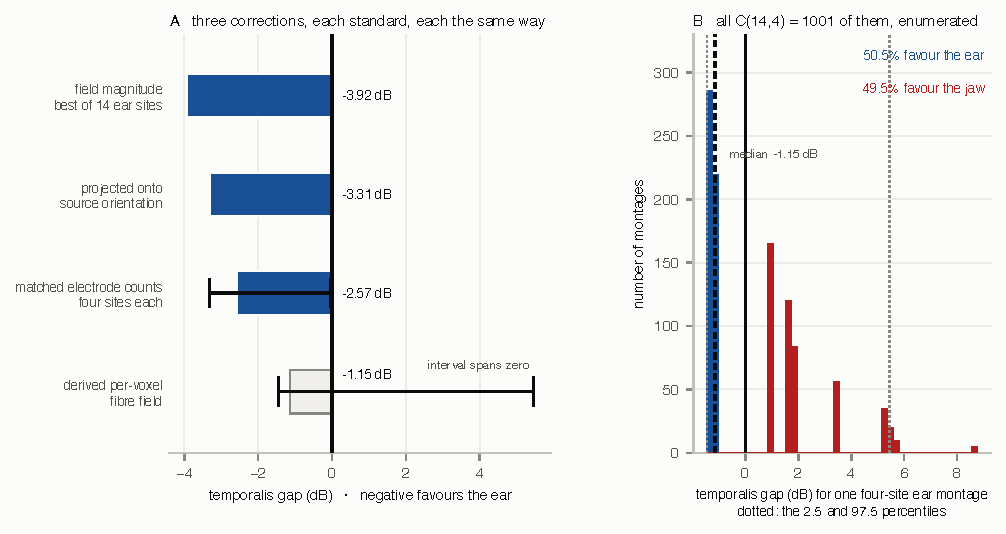
\includegraphics[width=\linewidth,height=0.42\textheight,keepaspectratio]{fig10_advantage_cascade.pdf}
\caption{How the retroauricular advantage dissolved. \emph{Left:} the temporalis gap at four stages, each read from the file that reproduces it: field magnitude against the best of fourteen ear sites, then projected onto source orientation, then at matched electrode counts, then under the fibre field derived from the label volume. Rules are matched-count intervals where one exists. Each correction is individually standard, none was applied in response to the result, and only the last interval spans zero. \emph{Right:} what that last interval is made of. The ear pool holds 14 sites and a montage takes 4, giving exactly C(14,4) = 1001 possible retroauricular montages, every one of which is enumerated here, so the histogram is the population, not a sample of it. Dotted lines are the 2.5 and 97.5 percentiles quoted as the interval; 28.6 per cent of montages attain the lower bound exactly, which is why that bound coincides with the floor.}
\end{figure}


Two features of this sequence are worth separating, because only one of them is
evidence. The \textbf{monotone} drift, every correction moving the same way, is
suggestive but not probative; corrections that each remove an optimistic
assumption will tend to move one way by construction. What is probative is that
the \textbf{final} step, the one that crosses zero, removes an assumption instead of
adding one, and was pre-committed (\S{}2.8) before the derived field existed. We do
not treat an effect as established when the assumption holding it up is one the
anatomy itself can replace.

We report this because the intermediate results were not obviously wrong. Each
was internally consistent, cleared its measurement floor, and reproduced an
a-priori anatomical prediction, the three muscles that appeared to favour the
ear are the three whose attachments sit at or near the temporal bone, which is
what one would predict, and which is what made the result convincing.

Figure 11 places temporalis against the other nine muscles on both robustness
axes at once, and marks the single row where the basis decides the verdict. It
is worth being explicit about that row, because Table 4 and the title of this
paper are computed on different bases, and a reader who sees only the table will
think they disagree.


\begin{figure}[htbp]
\centering
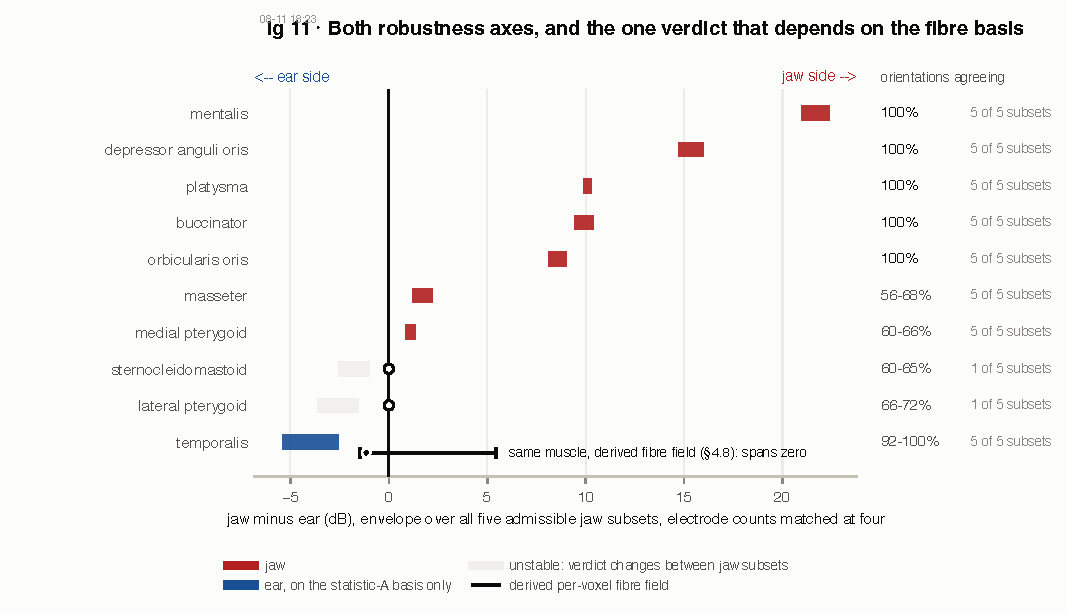
\includegraphics[width=\linewidth,height=0.42\textheight,keepaspectratio]{fig11_two_axis_envelope.pdf}
\caption{Both robustness axes, and the one verdict that depends on the basis. Table 4 drawn: one bar per muscle spanning the envelope over all five admissible jaw subsets, with electrode counts matched at four, coloured by verdict, against the orientation-agreement range on the right. Five muscles sit entirely on the jaw side on both axes. Two are unstable, changing verdict between jaw subsets, and their bars cross zero. Temporalis sits entirely on the ear side on the statistic-A basis used for Table 4, which takes the median over a uniform 200-direction orientation sweep. The black rule beneath it is the same comparison under the per-voxel fibre field derived from the label volume, which spans zero. It is the only row that carries a second rule, because it is the only muscle whose verdict depends on which basis is used, and \S{}4.8 gives the argument for preferring the derived field.}
\end{figure}


\begin{center}\rule{0.5\linewidth}{0.5pt}\end{center}

\subsection{Tables}\label{tables}

\textbf{Table 4, Which montage sees which muscle, on two robustness axes.} Gap in dB
between the jaw and retroauricular montages, positive favouring the jaw, taken
as the median over 200 source orientations of the per-orientation gap (statistic
A) against the four pre-registered retroauricular sites. Electrode counts are
matched at 4 per montage. Because 5 jaw sites are admissible and the comparison
takes 4, every value is reported as the envelope over all 5 admissible subsets
and not for one chosen subset. Rows marked unstable change verdict between
subsets and are described in the text. \emph{Site-robust} asks whether a random draw
of four of the fourteen ear sites still excludes zero. \emph{Orientation agreement}
is the fraction of sampled orientations agreeing with the median verdict. The
temporalis verdict is specific to this basis and does not hold under the derived
fibre field; see \S{}4.8 and Figure 11.

{\def\LTcaptype{none} % do not increment counter
\begin{longtable}[]{@{}
  >{\raggedright\arraybackslash}p{\dimexpr(\linewidth - 10\tabcolsep)*2000/10000\relax}
  >{\raggedright\arraybackslash}p{\dimexpr(\linewidth - 10\tabcolsep)*1700/10000\relax}
  >{\raggedright\arraybackslash}p{\dimexpr(\linewidth - 10\tabcolsep)*1200/10000\relax}
  >{\raggedright\arraybackslash}p{\dimexpr(\linewidth - 10\tabcolsep)*1600/10000\relax}
  >{\raggedright\arraybackslash}p{\dimexpr(\linewidth - 10\tabcolsep)*3500/10000\relax}@{}}
\toprule\noalign{}
\begin{minipage}[b]{\linewidth}\raggedright
Muscle
\end{minipage} & \begin{minipage}[b]{\linewidth}\raggedright
Gap (dB), envelope over subsets
\end{minipage} & \begin{minipage}[b]{\linewidth}\raggedright
Site-robust
\end{minipage} & \begin{minipage}[b]{\linewidth}\raggedright
Orientation agreement
\end{minipage} & \begin{minipage}[b]{\linewidth}\raggedright
Verdict
\end{minipage} \\
\midrule\noalign{}
\endhead
\bottomrule\noalign{}
\endlastfoot
mentalis & +20.98 to +22.40 & yes, all 5 & 100.0 \% & \textbf{jaw, robust on both axes} \\
depressor anguli oris & +14.70 to +15.98 & yes, all 5 & 100.0 \% & \textbf{jaw, robust on both axes} \\
buccinator & +9.45 to +10.39 & yes, all 5 & 100.0 \% & \textbf{jaw, robust on both axes} \\
platysma & +9.90 to +10.27 & yes, all 5 & 100.0 \% & \textbf{jaw, robust on both axes} \\
orbicularis oris & +8.11 to +9.02 & yes, all 5 & 100.0 \% & \textbf{jaw, robust on both axes} \\
masseter & +1.20 to +2.22 & yes, all 5 & 56.0--68.5 \% & \textbf{jaw, site-robust but orientation-dependent} \\
medial pterygoid & +0.86 to +1.33 & yes, all 5 & 59.5--66.5 \% & \textbf{jaw, site-robust but orientation-dependent} \\
sternocleidomastoid & \textminus{}2.53 to \textminus{}0.97 & 1 of 5 & 60.5--65.0 \% & \textbf{unstable across subsets} \\
lateral pterygoid & \textminus{}3.61 to \textminus{}1.53 & 1 of 5 & 65.5--72.0 \% & \textbf{unstable across subsets} \\
temporalis & \textminus{}5.42 to \textminus{}2.57 & yes, all 5 & 92.0--100.0 \% & \textbf{ear, robust on both axes} \\
\end{longtable}
}

No jaw site is preferred by the design over any other, so rather than select one
4-site subset the comparison is run over all 5 admissible subsets and reported as
an envelope. 5 of 10 muscles favour the jaw montage on both robustness axes in
every subset, spanning 8.11 to 22.40 dB. One muscle, temporalis, favours the
retroauricular montage on both axes on this basis, in every subset. That verdict
does not survive a change of basis. Statistic A takes the median over a uniform
orientation sweep, and under the per-voxel fibre field derived from the label
volume the same comparison gives \textminus{}1.15 dB with an interval of {[}\textminus{}1.45, +5.46{]}
that spans zero (\S{}4.8, Figure 11). Under the derived field, no muscle favours the
retroauricular montage on both axes.

8 muscles return an identical verdict in all 5 subsets. Two do not. Lateral
pterygoid gives no resolvable preference across four subsets (\textminus{}1.53 to \textminus{}1.59 dB)
and \textminus{}3.61 dB in the fifth; sternocleidomastoid gives \textminus{}0.97 to \textminus{}1.44 dB across
four and \textminus{}2.53 dB in the fifth. In both cases the deviating subset is the one
dropping \texttt{midjaw}, and in both cases the deviating value is site-robust but
orientation-dependent, with agreement of 72.0 and 65.0 per cent against the
90 per cent required for a robust preference. Neither reaches a retroauricular
preference on both axes, and neither is among the 5 muscles carrying the jaw
advantage. \texttt{midjaw} has the largest perpendicular clearance to the cut plane of
any jaw site at 63.76 mm; the instability follows from removing the site
furthest from the truncation, not one near it.

\textbf{Temporalis is reported here under the uniform orientation sweep, for
comparability with the other nine muscles.} Under the fibre field derived from
the label volume (\S{}2.5.1) it reads \textminus{}1.15 dB with a random-4 interval of
{[}\textminus{}1.45, +5.46{]}, which crosses zero, and that is the value the paper's conclusions
use (\S{}3.1, \S{}4.1). The two treatments disagree; the derived one governs because it
removes an assumption rather than adding one. This row shows what the
assumption-free treatment gives, so the dependence is visible, not buried.

\textbf{Table 5, Strongest single site for each articulator, and how well resolved it
is.} For each of the ten segmented articulators, the electrode with the largest
projected lead field under the isotropic model, its runner-up, and the margin
between them. Margins marked * are at or below 0.65 dB, the upper bound of the
95 \% CI on the electrode-meshing floor (\S{}2.7, row 6), so for those muscles the
identity of the strongest site is not resolved by this model. The final column
is what the table exists for: no articulator's runner-up sits in the other
montage, so site-level fragility does not propagate to the montage assignment.
These are single electrodes under an unmatched argmax, so the table records
where coupling is strongest and is not a montage recommendation; see \S{}4.4.
\texttt{earlobe\_ipsi} is solved but belongs to no montage and is excluded.

{\def\LTcaptype{none} % do not increment counter
\begin{longtable}[]{@{}
  >{\raggedright\arraybackslash}p{\dimexpr(\linewidth - 12\tabcolsep)*2000/10000\relax}
  >{\raggedright\arraybackslash}p{\dimexpr(\linewidth - 12\tabcolsep)*1800/10000\relax}
  >{\raggedright\arraybackslash}p{\dimexpr(\linewidth - 12\tabcolsep)*1000/10000\relax}
  >{\raggedright\arraybackslash}p{\dimexpr(\linewidth - 12\tabcolsep)*1800/10000\relax}
  >{\raggedright\arraybackslash}p{\dimexpr(\linewidth - 12\tabcolsep)*1300/10000\relax}
  >{\raggedright\arraybackslash}p{\dimexpr(\linewidth - 12\tabcolsep)*2100/10000\relax}@{}}
\toprule\noalign{}
\begin{minipage}[b]{\linewidth}\raggedright
Articulator
\end{minipage} & \begin{minipage}[b]{\linewidth}\raggedright
Best single site
\end{minipage} & \begin{minipage}[b]{\linewidth}\raggedright
Montage
\end{minipage} & \begin{minipage}[b]{\linewidth}\raggedright
Runner-up
\end{minipage} & \begin{minipage}[b]{\linewidth}\raggedright
Margin (dB)
\end{minipage} & \begin{minipage}[b]{\linewidth}\raggedright
Runner-up crosses montage
\end{minipage} \\
\midrule\noalign{}
\endhead
\bottomrule\noalign{}
\endlastfoot
masseter & buccal & jaw & mental & 0.86 & no \\
temporalis & cg01 & ear & cg02 & 0.71 & no \\
medial pterygoid & hyoid & jaw & submaxillary & 0.88 & no \\
lateral pterygoid & pre-tragus & ear & cg10 & 0.85 & no \\
orbicularis oris & mental & jaw & buccal & 1.02 & no \\
buccinator & mental & jaw & submental (mid) & 0.88 & no \\
mentalis & mental & jaw & submental (mid) & 0.27 * & no \\
depressor anguli oris & submental (mid) & jaw & mental & 0.15 * & no \\
platysma & hyoid & jaw & submental (mid) & 0.37 * & no \\
sternocleidomastoid & post-lobule & ear & cg08 & 0.03 * & no \\
\end{longtable}
}

\FloatBarrier
\subsection{Data and code availability}\label{data-and-code-availability}

All analysis code, electrode definitions, conductivity assignments and result
tables are maintained in a public repository, with the pre-registration commits
of \S{}2.8 citable by hash. The repository link is withheld for anonymous review
and will be restored in the final version. The MIDA model itself cannot be
redistributed under its licence and must be obtained from the IT'IS Foundation;
the repository documents the one manual step.

\FloatBarrier
\subsection{References}\label{references}

1. An, et al.~(2025). ID.EARS: One-Ear EEG Device with Biosignal Noise for Real-Time Gesture Recognition and Various Interactions. \emph{CHI '25}, 1--18. doi:10.1145/3706598.3714185
2. Avramidou, et al.~(2024). From Ear-EEG to Ear-ExG: The Jaw Artifact is a Keeper. \emph{DSAI '24}.
3. Debener, S., et al.~(2015). Unobtrusive ambulatory EEG using a smartphone and flexible printed electrodes around the ear. \emph{Sci Rep} 5:16743. doi:10.1038/srep16743
4. De Luca, C. J., et al.~(2012). Inter-electrode spacing of surface EMG sensors. \emph{J Biomech} 45(3):555--561. doi:10.1016/j.jbiomech.2011.11.010
5. Gaddy, D., \& Klein, D. (2020). Digital Voicing of Silent Speech. \emph{EMNLP}, 5521--5530. doi:10.18653/v1/2020.emnlp-main.445
6. Goncharova, I. I., et al.~(2003). EMG contamination of EEG: spectral and topographical characteristics. \emph{Clin Neurophysiol}.
7. Harmening, N., Klug, M., Gramann, K., \& Miklody, D. (2022). HArtMuT, modeling eye and muscle contributors in neuroelectric imaging. \emph{J Neural Eng} 19(6):066041. doi:10.1088/1741-2552/aca8ce
8. Iacono, M. I., et al.~(2015). MIDA: A Multimodal Imaging-Based Detailed Anatomical Model of the Human Head and Neck. \emph{PLOS ONE}. doi:10.1371/journal.pone.0124126
9. Kappel, S. L., Makeig, S., \& Kidmose, P. (2019). Ear-EEG Forward Models: Improved Head-Models for Ear-EEG. \emph{Front Neurosci} 13:943. doi:10.3389/fnins.2019.00943
10. Kapur, A., Kapur, S., \& Maes, P. (2018). AlterEgo: A Personalized Wearable Silent Speech Interface. \emph{IUI '18}, 43--53. doi:10.1145/3172944.3172977
11. Kuiken, T. A., Lowery, M. M., \& Stoykov, N. S. (2003). The effect of subcutaneous fat on myoelectric signal amplitude and cross-talk. \emph{Prosthet Orthot Int} 27(1):48--54. doi:10.3109/03093640309167976
12. Maksymenko, K., Deslauriers-Gauthier, S., \& Farina, D. (2021). Ultra fast and highly realistic numerical modelling of surface EMG. \emph{bioRxiv}.
13. Meiser, A., Knoll, J., \& Bleichner, M. G. (2024). High-density ear-EEG for understanding ear-centered EEG. \emph{J Neural Eng} 21(1):016001. doi:10.1088/1741-2552/ad1783
14. Mesin, L. (2020). Crosstalk in surface electromyogram: literature review and some insights. \emph{Phys Eng Sci Med} 43(2):481--492. doi:10.1007/s13246-020-00868-1
15. Sato, W., \& Kochiyama, T. (2023). Crosstalk in Facial EMG and Its Reduction Using ICA. \emph{Sensors} 23:2720.
16. Saturnino, G. B., Madsen, K. H., \& Thielscher, A. (2019). Electric field simulations for transcranial brain stimulation using FEM: an efficient implementation and error analysis. \emph{J Neural Eng} 16(6):066032. doi:10.1088/1741-2552/ab41ba
17. Thielscher, A., Antunes, A., \& Saturnino, G. B. (2015). Field modeling for transcranial magnetic stimulation: a useful tool to understand the physiological effects of TMS? \emph{EMBC 2015}, 222--225. doi:10.1109/EMBC.2015.7318340
18. Wand, M., \& Schultz, T. (2011). Session-Independent EMG-Based Speech Recognition. \emph{BIOSIGNALS 2011}, 295--300. doi:10.5220/0003169702950300
19. Yao, D., et al.~(2019). Which Reference Should We Use for EEG and ERP practice? \emph{Brain Topogr}.
20. Yarici, M., Thornton, M., \& Mandic, D. P. (2023). Ear-EEG sensitivity modeling for neural sources and ocular artifacts. \emph{Front Neurosci} 16:997377. doi:10.3389/fnins.2022.997377

\FloatBarrier
\subsection{Appendix A: Extended methods detail}\label{appendix-a-extended-methods-detail}

\subsubsection{A.1 Detail for \S{}2.1 Head model}\label{a.1-detail-for-2.1-head-model}

\textbf{Boundary.} The MIDA head model is truncated inferiorly on a planar cut, and
that face is treated as an insulating (homogeneous Neumann) boundary. The face
is fitted from 18,818 boundary triangles with unit normal {[}\textminus{}0.03336, \textminus{}0.03236,
\textminus{}0.99892{]}, tilted 2.664\textdegree{} off the RAS S axis, passing through (\textminus{}2.301, 23.112,
\textminus{}115.600) mm; residual RMS about the fit is 0.073 mm. Because the plane is
tilted it has no single S coordinate: the face spans S = \textminus{}122.07 to \textminus{}110.17 mm
across its lateral extent, and the mesh S minimum, \textminus{}122.167 mm, is a corner of
that face, not the location of the cut. All boundary clearances reported here
are perpendicular distances to this plane, not differences in S.

The cut plane is not fitted to an assumed orientation. Its normal recovers the
MIDA label volume's own superior voxel axis, read from the NIfTI affine as
{[}0.03335, 0.03240, 0.99892{]} at 2.665\textdegree{} from RAS +S with a 0.500 mm step, agreeing
with the fitted normal to 0.0026\textdegree{}. The truncation therefore lies on a voxel plane
of the source segmentation. No node of the mesh lies more than 0.276 mm outside
the fitted plane, so it is the outer boundary and carries the insulating
condition.

\textbf{Mesh validation.} Every tag present in the mesh carries an assigned
conductivity, verified by enumeration (0 of 118 volume tags uncovered). MIDA's
own labels 100--116 lie inside SimNIBS's reserved electrode-rubber range 100--499
and are correct only because Table 1 names each explicitly; this is checked at
run time.

\subsubsection{A.2 Detail for \S{}2.2 Conductivity assignment}\label{a.2-detail-for-2.2-conductivity-assignment}

Provenance is mixed, deliberately, and stated per row. SimNIBS 4.6 defaults are
used for the primary head tissues, skin, fat, compact and cancellous bone, grey
and white matter, CSF, blood, eye, muscle, cartilage, air, because these are
the conventional head-modelling values and using them keeps this model
comparable with the existing EEG and tDCS forward-model literature. The IT'IS
Low Frequency database v4.2 (DOI 10.13099/VIP21000-04-2) supplies every tissue
SimNIBS carries no default for. A small number of assignments are judgement,
marked as such in Table 1, where MIDA segments a structure IT'IS does not list
separately; each carries a note giving the reasoning.

Insensitivity to that choice was measured, not assumed. Solving at
$\sigma$\_air = 10\textsuperscript{\textminus6}, 10\textsuperscript{\textminus5}, 10\textsuperscript{\textminus4} and 10\textsuperscript{\textminus3} S/m on identical geometry, the largest
departure over the ten muscle compartments from the 10\textsuperscript{\textminus6} baseline is 0.007 dB at
10\textsuperscript{\textminus5}, 0.069 dB at 10\textsuperscript{\textminus4} and 0.467 dB at 10\textsuperscript{\textminus3}. The result is therefore
insensitive across 10\textsuperscript{\textminus6} to 10\textsuperscript{\textminus4}, where the largest departure sits roughly four
times below the measured noise floor of 0.27 dB. Departure begins at 10\textsuperscript{\textminus3}, where
it reaches 1.7\texttimes{} the floor and concentrates in the compartments nearest the oral
and nasal cavities (mentalis \textminus{}0.467, orbicularis oris \textminus{}0.433) while remote
compartments are essentially unmoved (temporalis \textminus{}0.029, lateral pterygoid
\textminus{}0.009). The operating value sits two decades inside the insensitive range.

\subsubsection{A.3 Detail for \S{}2.3 Electrode placement}\label{a.3-detail-for-2.3-electrode-placement}

Target localisation uses a hybrid of centroid-interior and minimum-distance, for
a geometric reason. For a compact compartment the centroid is a good interior
representative. For a non-convex compartment the centroid need not lie inside
the compartment at all, the mandible is the clear case, since it is an arch and
the centroid of an arch lies in the space the arch encloses, so an electrode
placed over that point would sit over the floor of the mouth. Where a
compartment's centroid does not lie within the compartment, the site is instead
defined by minimum distance from the skin surface to the compartment. Which rule
applied to which site is recorded per row.

The midline is derived, not assumed to be R = 0: MIDA's head is not perfectly
centred in its own voxel grid, so the anatomical midline is computed from the
mandible label and midline sites are placed relative to that plane. Per-site
depth, skin surface to target compartment along the placement ray, is reported
for every site.

One position is withheld. \texttt{throat\_scm} is recorded as held with blank
coordinates: MIDA's sternocleidomastoid is truncated at the cut face, which
biases its centroid posteriorly, so no defensible automatic placement exists.
Every consumer skips it instead of substituting a nearby label.

\subsubsection{A.4 Detail for \S{}2.5 Fibre orientation}\label{a.4-detail-for-2.5-fibre-orientation}

Two further restrictions apply and both bite. A compartment must be individually
segmented to carry a per-compartment axis, which excludes the six pooled
suprahyoid and tongue muscles. And each axis must pass a bilateral
mirror-symmetry test: MIDA assigns one label to both sides of a paired muscle,
so PCA on the pooled voxel cloud returns the left--right separation between the
two bellies rather than the fibre direction along either. Axes are therefore
computed per side and required to be mirror images in x. Three compartments were
tested against it, that being the entire population which is both individually
segmented and PCA-defensible; it is not a gate the remaining seven passed.
Sternocleidomastoid
passes at \textbar dot\textbar{} = 0.98 and medial pterygoid at 1.000; mentalis fails at 0.215,
its two fragments having a right-side elongation ratio of 1.07, so no long axis
exists to find, and it receives no tensor.

The anisotropic condition is solved on the isotropic run's own mesh with only
the conductivity field replaced. SimNIBS re-meshes electrodes on each session
and two sessions of the same montage can differ, so solving on the identical
mesh removes electrode realisation, comparable in size to the effect being
measured, from the comparison.

\subsubsection{A.5 Detail for \S{}2.6 Validation}\label{a.5-detail-for-2.6-validation}

\textbf{Reciprocity on the head mesh.} The identity is verified on the real geometry
by solving a montage and its polarity-swapped counterpart and requiring
L(A$\rightarrow$B) = \textminus{}L(B$\rightarrow$A). On identical discretisations the residual is 7.5 \texttimes{} 10\textsuperscript{\textminus6} of
\textbar L\textbar, i.e.~6.5 \texttimes{} 10\textsuperscript{\textminus5} dB --- four orders of magnitude below the measured per-site
noise floor.

\textbf{Four physical invariants}, computed from the field alone and requiring no
solver internals: (1) flux through a closed surface around an electrode is
radius-independent; (2) net current through a surface enclosing the whole domain
is zero; (3) doubling the injected current doubles the field exactly; (4)
swapping source and sink negates the field. Invariant 1 uses an exact tet-patch
integral in which flux is integrated over the interior cut of a patch of
tetrahedra using the mesh's own faces as the quadrature, so enclosure and
orientation are exact by construction (the patch surface closes to 1.2 \texttimes{} 10\textsuperscript{\textminus16}
of its own area) and no inside/outside point test is required. A stationary
plateau across radii 25--75 mm is required before any value is used. Invariants 1
and 2 run on every solve; 3 and 4 require paired solves and run on the first and
last of a batch. All guards collect and raise once with every failure instead of
raising on the first.

\textbf{Convergence.} RDM against the analytic sphere was fitted across three mesh
densities, giving a convergence exponent p = 0.980, consistent with the
theoretical p $\approx$ 1 expected for a gradient quantity in a first-order FEM. This is
stated as consistency, not corroboration: three data points fitted with three
free parameters is an exact fit by construction, so p is determined
algebraically and the residual carries no goodness-of-fit information.

\textbf{Guard tests.} Two meta-tests protect the validation itself. A coverage test
resolves, from the abstract syntax tree, that every production script actually
invokes its guards. A synthetic-fire test requires each guard to fail on a
purpose-built input that fails that guard and nothing else, with a clean control
that trips none; this detects a guard rendered unreachable by an earlier guard's
raise, which a coverage test cannot see.

\subsubsection{A.6 Detail for \S{}2.8 Reproducibility and pre-registration}\label{a.6-detail-for-2.8-reproducibility-and-pre-registration}

One qualification, because the claim is otherwise stronger than the repository
delivers. \texttt{data/mida\_headneck.msh} is not under version control, and \texttt{meshmesh}
is not deterministic: the same label volume and the same script produced
12,294,185 tetrahedra on one machine and 12,587,663 on another. A clean checkout
therefore rebuilds a mesh that is not the one these numbers came from, and the
cut-plane guard in \texttt{config.cut\_plane()} will refuse it by design, since the
plane is fitted to a specific mesh and verified by hash. Reproducing the
pipeline is possible from a clean checkout; reproducing these exact values needs
the mesh, and term 10 of the error budget quantifies what that difference is
worth.

A published table with no generating script is not a result yet. Two tables in
this study (\texttt{04h\_matched\_counts.csv}, \texttt{04j\_two\_axis\_verdict.csv}) were initially
produced interactively rather than by a script in \texttt{src/}. They could not be
regenerated from a clean checkout, and they drifted out of step with the
renormalisation specified above. That suspicion proved false; they were correct,
and an attempt to ``correct'' them applied the renormalisation a second time and
moved nine published numbers by up to 1.04 dB before it was caught by checking
the upstream script. The episode is reported because the failure mode is
general: a table with no generating script cannot be audited by reading it,
since every number in it is internally consistent whether or not it is right.
Both are now generated by \texttt{src/04h\_matched\_counts.py}, and no quantity enters
the manuscript except from a file some script in \texttt{src/} writes.

\subsection{Appendix B: Tables 1, 2 and 3}\label{appendix-b-tables-1-2-and-3}

\textbf{Table 1, Tissue conductivities.} All 116 MIDA labels with assigned
conductivity, source (SimNIBS 4.6 default / IT'IS LF v4.2 / judgement),
frequency, plausible range for judgement rows, volume fraction and minimum
distance to the nearest electrode. Sorted by volume fraction \texttimes{} proximity.
{[}\texttt{results/01\_table1\_conductivities.csv}{]}

{\def\LTcaptype{none} % do not increment counter
\begin{landscape}
\let\footnotesize\scriptsize
\begin{longtable}[]{@{}
  >{\raggedright\arraybackslash}p{\dimexpr(\linewidth - 22\tabcolsep)*300/10000\relax}
  >{\raggedright\arraybackslash}p{\dimexpr(\linewidth - 22\tabcolsep)*1400/10000\relax}
  >{\raggedright\arraybackslash}p{\dimexpr(\linewidth - 22\tabcolsep)*1000/10000\relax}
  >{\raggedright\arraybackslash}p{\dimexpr(\linewidth - 22\tabcolsep)*1400/10000\relax}
  >{\raggedright\arraybackslash}p{\dimexpr(\linewidth - 22\tabcolsep)*400/10000\relax}
  >{\raggedright\arraybackslash}p{\dimexpr(\linewidth - 22\tabcolsep)*720/10000\relax}
  >{\raggedright\arraybackslash}p{\dimexpr(\linewidth - 22\tabcolsep)*680/10000\relax}
  >{\raggedright\arraybackslash}p{\dimexpr(\linewidth - 22\tabcolsep)*1550/10000\relax}
  >{\raggedright\arraybackslash}p{\dimexpr(\linewidth - 22\tabcolsep)*620/10000\relax}
  >{\raggedright\arraybackslash}p{\dimexpr(\linewidth - 22\tabcolsep)*450/10000\relax}
  >{\raggedright\arraybackslash}p{\dimexpr(\linewidth - 22\tabcolsep)*1480/10000\relax}@{}}
\toprule\noalign{}
\begin{minipage}[b]{\linewidth}\raggedright
\#
\end{minipage} & \begin{minipage}[b]{\linewidth}\raggedright
MIDA structure
\end{minipage} & \begin{minipage}[b]{\linewidth}\raggedright
Assigned tissue
\end{minipage} & \begin{minipage}[b]{\linewidth}\raggedright
$\sigma$ (S/m)
\end{minipage} & \begin{minipage}[b]{\linewidth}\raggedright
f (Hz)
\end{minipage} & \begin{minipage}[b]{\linewidth}\raggedright
Source
\end{minipage} & \begin{minipage}[b]{\linewidth}\raggedright
Assignment
\end{minipage} & \begin{minipage}[b]{\linewidth}\raggedright
Plausible range (S/m)
\end{minipage} & \begin{minipage}[b]{\linewidth}\raggedright
Volume fraction
\end{minipage} & \begin{minipage}[b]{\linewidth}\raggedright
Min. distance (mm)
\end{minipage} & \begin{minipage}[b]{\linewidth}\raggedright
Note
\end{minipage} \\
\midrule\noalign{}
\endhead
\bottomrule\noalign{}
\endlastfoot
51 & Epidermis/Dermis & skin & 0.465 & 100.0 & SimNIBS 4.6 default & lookup & & 0.059625 & 0.7 & \\
62 & Subcutaneous Adipose Tissue & fat & 0.025 & 100.0 & SimNIBS 4.6 default & lookup & & 0.097494 & 1.65 & \\
43 & Adipose Tissue & fat & 0.025 & 100.0 & SimNIBS 4.6 default & lookup & & 0.11177 & 2.45 & \\
63 & Muscle - Temporalis/Temporoparietalis & muscle\_iso & 0.355 & 100.0 & SimNIBS 4.6 default & lookup & & 0.028682 & 2.55 & \\
40 & Skull & bone\_compact & 0.008 & 100.0 & SimNIBS 4.6 default & lookup & & 0.045984 & 3.94 & \\
38 & Muscle (General) & muscle\_iso & 0.355 & 100.0 & SimNIBS 4.6 default & lookup & & 0.058249 & 5.19 & \\
67 & Muscle - Splenius Capitis & muscle\_iso & 0.355 & 100.0 & SimNIBS 4.6 default & lookup & & 0.008552 & 2.3 & \\
68 & Muscle - Sternocleidomastoid & muscle\_iso & 0.355 & 100.0 & SimNIBS 4.6 default & lookup & & 0.009119 & 2.55 & \\
10 & Brain Gray Matter & grey\_matter & 0.275 & 100.0 & SimNIBS 4.6 default & lookup & & 0.110101 & 11.19 & \\
54 & Skull Outer Table & bone\_compact & 0.008 & 100.0 & SimNIBS 4.6 default & lookup & & 0.020085 & 5.5 & skull outer table is cortical bone \\
12 & Brain White Matter & white\_matter & 0.126 & 100.0 & SimNIBS 4.6 default & lookup & & 0.116885 & 14.06 & \\
35 & Ear Auricular Cartilage (Pinna) & cartilage & 0.17 & 100.0 & SimNIBS 4.6 default & lookup & & 0.001851 & 1.87 & \\
52 & Skull Diploë & bone\_cancellous & 0.025 & 100.0 & SimNIBS 4.6 default & lookup & & 0.02604 & 8.08 & diploe is cancellous bone \\
32 & CSF General & csf & 1.79 & 100.0 & SimNIBS 4.6 default & lookup & & 0.046232 & 10.78 & \\
36 & Mandible & Mandible & 0.00630199709513435 & 100.0 & IT'IS LF v4.2 & lookup & 0.001851851851851852 to 0.0091 & 0.010394 & 5.53 & \\
89 & Parotid Gland & Salivary Gland & 0.5585997222608695 & 100.0 & IT'IS LF v4.2 & lookup & 0.435631853 to 0.743 & 0.011107 & 6.4 & \\
53 & Skull Inner Table & bone\_compact & 0.008 & 100.0 & SimNIBS 4.6 default & lookup & & 0.016097 & 8.03 & skull inner table is cortical bone \\
60 & Muscle - Platysma & muscle\_iso & 0.355 & 100.0 & SimNIBS 4.6 default & lookup & & 0.002112 & 3.05 & \\
1 & Dura & Dura & 0.06 & 100.0 & IT'IS LF v4.2 & lookup & 0.0006 to 0.06 & 0.020207 & 9.76 & \\
66 & Muscle - Masseter & muscle\_iso & 0.355 & 100.0 & SimNIBS 4.6 default & lookup & & 0.012406 & 8.27 & \\
72 & Muscle - Depressor Anguli Oris & muscle\_iso & 0.355 & 100.0 & SimNIBS 4.6 default & lookup & & 0.001387 & 4.39 & \\
98 & Tendon - Temporalis Tendon & Tendon\textbackslash Ligament & 0.3675772277227722 & 100.0 & IT'IS LF v4.2 & lookup & 0.3675772277227722 to 0.3675772277227722 & 0.001796 & 5.24 & \\
37 & Mucosa & Mucous Membrane & 0.4610075264456888 & 100.0 & IT'IS LF v4.2 & lookup & 0.1 to 0.726 & 0.01077 & 13.51 & \\
2 & Cerebellum Gray Matter & Cerebellum & 0.5766124444444444 & 100.0 & IT'IS LF v4.2 & judgement & 0.48 to 0.646504 & 0.020041 & 19.16 & IT'IS carries one Cerebellum entry, not split into grey and white matter \\
25 & Blood Veins & blood & 0.7 & 100.0 & SimNIBS 4.6 default & lookup & & 0.007009 & 11.89 & \\
31 & Air Internal - Nasal/Pharynx & air & 1e-06 & 100.0 & SimNIBS 4.6 default & lookup & & 0.010299 & 15.1 & \\
73 & Muscle - Depressor Labii & muscle\_iso & 0.355 & 100.0 & SimNIBS 4.6 default & lookup & & 0.000703 & 4.35 & \\
42 & Tongue & muscle\_iso & 0.355 & 100.0 & SimNIBS 4.6 default & lookup & & 0.015368 & 25.5 & \\
41 & Teeth & Tooth & 0.00630199709513435 & 100.0 & IT'IS LF v4.2 & lookup & 0.001851851851851852 to 0.0091 & 0.004493 & 14.68 & \\
65 & Muscle - Lateral Pterygoid & muscle\_iso & 0.355 & 100.0 & SimNIBS 4.6 default & lookup & & 0.004071 & 14.04 & \\
9 & Cerebellum White Matter & Cerebellum & 0.5766124444444444 & 100.0 & IT'IS LF v4.2 & judgement & 0.48 to 0.646504 & 0.011022 & 24.46 & same single Cerebellum entry; MIDA splits it, IT'IS does not \\
84 & Muscle - Buccinator & muscle\_iso & 0.355 & 100.0 & SimNIBS 4.6 default & lookup & & 0.00209 & 11.06 & \\
88 & Submandibular Gland & Salivary Gland & 0.5585997222608695 & 100.0 & IT'IS LF v4.2 & lookup & 0.435631853 to 0.743 & 0.007198 & 21.79 & \\
24 & Blood Arteries & blood & 0.7 & 100.0 & SimNIBS 4.6 default & lookup & & 0.003119 & 14.6 & \\
97 & Air Internal - Oral Cavity & air & 1e-06 & 100.0 & SimNIBS 4.6 default & lookup & & 0.005035 & 19.7 & \\
71 & Muscle - Mentalis & muscle\_iso & 0.355 & 100.0 & SimNIBS 4.6 default & lookup & & 0.000264 & 5.14 & \\
75 & Muscle - Orbicularis Oris & muscle\_iso & 0.355 & 100.0 & SimNIBS 4.6 default & lookup & & 0.002573 & 17.57 & \\
61 & Tendon - Galea Aponeurotica & Tendon\textbackslash Ligament & 0.3675772277227722 & 100.0 & IT'IS LF v4.2 & lookup & 0.3675772277227722 to 0.3675772277227722 & 0.009629 & 35.75 & \\
81 & Muscle - Medial Pterygoid & muscle\_iso & 0.355 & 100.0 & SimNIBS 4.6 default & lookup & & 0.004639 & 28.94 & \\
85 & Ear Auditory Canal & air & 1e-06 & 100.0 & SimNIBS 4.6 default & judgement & 1e-06 to 1e-06 & 0.000326 & 7.76 & external auditory canal, air-filled and non-collapsing in a healthy ear. No range: cerumen occlusion has no sourced conductivity and is not modelled. \\
83 & Muscles - Risorius & muscle\_iso & 0.355 & 100.0 & SimNIBS 4.6 default & lookup & & 0.001301 & 15.97 & \\
78 & Muscle - Zygomaticus Major & muscle\_iso & 0.355 & 100.0 & SimNIBS 4.6 default & lookup & & 0.000877 & 14.11 & \\
90 & Sublingual Gland & Salivary Gland & 0.5585997222608695 & 100.0 & IT'IS LF v4.2 & lookup & 0.435631853 to 0.743 & 0.001167 & 16.47 & \\
44 & Vertebra - C1 (atlas) & Vertebrae & 0.00630199709513435 & 100.0 & IT'IS LF v4.2 & lookup & 0.001851851851851852 to 0.0091 & 0.002563 & 32.04 & \\
80 & Muscle - Levator Scapulae & muscle\_iso & 0.355 & 100.0 & SimNIBS 4.6 default & lookup & & 0.00312 & 37.36 & \\
28 & Air Internal - Maxillary Sinus & air & 1e-06 & 100.0 & SimNIBS 4.6 default & lookup & & 0.002866 & 38.48 & \\
6 & CSF Ventricles & csf & 1.79 & 100.0 & SimNIBS 4.6 default & lookup & & 0.002828 & 40.4 & \\
108 & Cranial Nerve V3 - Mandibular Division & Nerve & 0.3479543931346832 & 100.0 & IT'IS LF v4.2 & lookup & 0.06435 to 0.85244 & 0.000178 & 10.32 & \\
45 & Vertebra - C2 (axis) & Vertebrae & 0.00630199709513435 & 100.0 & IT'IS LF v4.2 & lookup & 0.001851851851851852 to 0.0091 & 0.003609 & 46.69 & \\
79 & Muscle - Orbicularis Oculi & muscle\_iso & 0.355 & 100.0 & SimNIBS 4.6 default & lookup & & 0.002336 & 42.38 & \\
57 & Eye Vitreous & eye & 1.5 & 100.0 & SimNIBS 4.6 default & lookup & & 0.003046 & 48.53 & \\
70 & Muscle - Trapezius & muscle\_iso & 0.355 & 100.0 & SimNIBS 4.6 default & lookup & & 0.003802 & 54.53 & \\
8 & Putamen & Brain (Grey Matter) & 0.4190548817650446 & 100.0 & IT'IS LF v4.2 & judgement & 0.06 to 0.83 & 0.002291 & 43.71 & deep grey nucleus, no IT'IS entry \\
116 & Thalamus & Thalamus & 0.475 & 100.0 & IT'IS LF v4.2 & lookup & 0.475 to 0.475 & 0.003147 & 52.57 & \\
30 & Air Internal - Mastoid & air & 1e-06 & 100.0 & SimNIBS 4.6 default & lookup & & 0.000331 & 17.13 & \\
46 & Vertebra - C3 & Vertebrae & 0.00630199709513435 & 100.0 & IT'IS LF v4.2 & lookup & 0.001851851851851852 to 0.0091 & 0.001957 & 42.31 & \\
47 & Vertebra - C4 & Vertebrae & 0.00630199709513435 & 100.0 & IT'IS LF v4.2 & lookup & 0.001851851851851852 to 0.0091 & 0.001857 & 41.6 & \\
14 & Brainstem Pons & Pons & 0.558392 & 100.0 & IT'IS LF v4.2 & lookup & 0.369 to 0.747784 & 0.003179 & 55.19 & \\
48 & Vertebra - C5 & Vertebrae & 0.00630199709513435 & 100.0 & IT'IS LF v4.2 & lookup & 0.001851851851851852 to 0.0091 & 0.001935 & 44.13 & \\
39 & Nasal Septum (Cartilage) & cartilage & 0.17 & 100.0 & SimNIBS 4.6 default & lookup & & 0.002536 & 53.87 & \\
86 & Ear Pharyngotympanic Tube & air & 1e-06 & 100.0 & SimNIBS 4.6 default & judgement & 1e-06 to 0.4610075264456888 & 0.000275 & 19.25 & pharyngotympanic tube, normally collapsed and mucosa-lined, so the range spans an open air lumen to a collapsed mucosal one. \\
87 & Hyoid Bone & Bone (Cortical) & 0.00630199709513435 & 100.0 & IT'IS LF v4.2 & judgement & 0.001851851851851852 to 0.0091 & 0.000285 & 19.68 & IT'IS has no hyoid entry; hyoid is a small cortical-shelled bone \\
11 & Brainstem Midbrain & Midbrain & 0.35 & 100.0 & IT'IS LF v4.2 & lookup & 0.35 to 0.35 & 0.001911 & 52.96 & \\
5 & Hippocampus & Hippocampus & 0.4190548817650446 & 100.0 & IT'IS LF v4.2 & lookup & 0.06 to 0.83 & 0.001181 & 42.14 & \\
69 & Muscle - Occipitiofrontalis - Occipital Belly & muscle\_iso & 0.355 & 100.0 & SimNIBS 4.6 default & lookup & & 0.001319 & 48.94 & \\
77 & Muscle - Levator Labii Superioris & muscle\_iso & 0.355 & 100.0 & SimNIBS 4.6 default & lookup & & 0.000665 & 39.88 & \\
7 & Caudate Nucleus & Brain (Grey Matter) & 0.4190548817650446 & 100.0 & IT'IS LF v4.2 & judgement & 0.06 to 0.83 & 0.001439 & 60.08 & deep grey nucleus, no IT'IS entry \\
13 & Spinal Cord & Spinal Cord & 0.6109538492063492 & 100.0 & IT'IS LF v4.2 & lookup & 0.49734388 to 0.781544 & 0.001373 & 59.95 & \\
26 & Air Internal - Ethmoidal Sinus & air & 1e-06 & 100.0 & SimNIBS 4.6 default & lookup & & 0.0013 & 58.89 & \\
15 & Brainstem Medulla & Medulla Oblongata & 0.357 & 100.0 & IT'IS LF v4.2 & lookup & 0.357 to 0.357 & 0.001147 & 55.96 & \\
4 & Amygdala & Brain (Grey Matter) & 0.4190548817650446 & 100.0 & IT'IS LF v4.2 & judgement & 0.06 to 0.83 & 0.000689 & 45.28 & deep grey nucleus, no IT'IS entry \\
49 & Intervertebral Discs & Intervertebral Disc & 0.7392595578616339 & 100.0 & IT'IS LF v4.2 & lookup & 0.600084 to 1.433653433962262 & 0.000625 & 43.94 & \\
17 & Globus Pallidus & Brain (Grey Matter) & 0.4190548817650446 & 100.0 & IT'IS LF v4.2 & judgement & 0.06 to 0.83 & 0.000701 & 50.98 & deep grey nucleus, no IT'IS entry \\
56 & Eye Retina/Choroid/Sclera & eye & 1.5 & 100.0 & SimNIBS 4.6 default & lookup & & 0.000605 & 47.61 & \\
93 & Muscle - Lateral Rectus & muscle\_iso & 0.355 & 100.0 & SimNIBS 4.6 default & lookup & & 0.000321 & 43.46 & \\
82 & Muscle - Zygomaticus Minor & muscle\_iso & 0.355 & 100.0 & SimNIBS 4.6 default & lookup & & 0.000202 & 34.83 & \\
74 & Muscle - Nasalis & muscle\_iso & 0.355 & 100.0 & SimNIBS 4.6 default & lookup & & 0.000502 & 55.05 & \\
64 & Muscle - Occipitiofrontalis - Frontal Belly & muscle\_iso & 0.355 & 100.0 & SimNIBS 4.6 default & lookup & & 0.000978 & 79.26 & \\
29 & Air Internal - Sphenoidal Sinus & air & 1e-06 & 100.0 & SimNIBS 4.6 default & lookup & & 0.000422 & 61.16 & \\
92 & Muscle - Medial Rectus & muscle\_iso & 0.355 & 100.0 & SimNIBS 4.6 default & lookup & & 0.000348 & 56.19 & \\
27 & Air Internal - Frontal Sinus & air & 1e-06 & 100.0 & SimNIBS 4.6 default & lookup & & 0.000734 & 82.52 & \\
91 & Muscle - Superior Rectus & muscle\_iso & 0.355 & 100.0 & SimNIBS 4.6 default & lookup & & 0.000287 & 51.93 & \\
94 & Muscle - Inferior Rectus & muscle\_iso & 0.355 & 100.0 & SimNIBS 4.6 default & lookup & & 0.000257 & 51.05 & \\
34 & Ear Semicircular Canals & Cerebrospinal Fluid & 1.878999709695023 & 100.0 & IT'IS LF v4.2 & judgement & 1.13 to 3.186944 & 8.1e-05 & 29.26 & semicircular canal endolymph, as above \\
110 & Cranial Nerve VII - Facial & Nerve & 0.3479543931346832 & 100.0 & IT'IS LF v4.2 & lookup & 0.06435 to 0.85244 & 3.9e-05 & 24.13 & \\
111 & Cranial Nerve VIII - Vestibulocochlear & Nerve & 0.3479543931346832 & 100.0 & IT'IS LF v4.2 & lookup & 0.06435 to 0.85244 & 8.6e-05 & 36.94 & \\
103 & Cranial Nerve II - Optic & Nerve & 0.3479543931346832 & 100.0 & IT'IS LF v4.2 & lookup & 0.06435 to 0.85244 & 0.000181 & 53.91 & \\
112 & Cranial Nerve IX - Glossopharyngeal & Nerve & 0.3479543931346832 & 100.0 & IT'IS LF v4.2 & lookup & 0.06435 to 0.85244 & 7e-05 & 34.89 & \\
113 & Cranial Nerve X - Vagus & Nerve & 0.3479543931346832 & 100.0 & IT'IS LF v4.2 & lookup & 0.06435 to 0.85244 & 7.2e-05 & 35.79 & \\
16 & Nucleus Accumbens & Brain (Grey Matter) & 0.4190548817650446 & 100.0 & IT'IS LF v4.2 & judgement & 0.06 to 0.83 & 0.00022 & 63.6 & deep grey nucleus, no IT'IS entry \\
59 & Eye Aqueous & eye & 1.5 & 100.0 & SimNIBS 4.6 default & lookup & & 0.000194 & 62.68 & \\
21 & Hypothalamus & Hypothalamus & 0.4190548817650446 & 100.0 & IT'IS LF v4.2 & lookup & 0.06 to 0.83 & 0.000234 & 69.16 & \\
95 & Muscle - Superior Oblique & muscle\_iso & 0.355 & 100.0 & SimNIBS 4.6 default & lookup & & 0.000162 & 61.72 & \\
96 & Muscle - Inferior Oblique & muscle\_iso & 0.355 & 100.0 & SimNIBS 4.6 default & lookup & & 0.000106 & 51.13 & \\
100 & Cerebral Peduncles & Brain (White Matter) & 0.3479543931346832 & 100.0 & IT'IS LF v4.2 & judgement & 0.06435 to 0.85244 & 0.000105 & 55.28 & myelinated tract \\
33 & Ear Cochlea & Cerebrospinal Fluid & 1.878999709695023 & 100.0 & IT'IS LF v4.2 & judgement & 1.13 to 3.186944 & 4.5e-05 & 36.44 & cochlear perilymph is CSF-like; IT'IS has no inner-ear fluid entry \\
106 & Cranial Nerve V - Trigeminal & Nerve & 0.3479543931346832 & 100.0 & IT'IS LF v4.2 & lookup & 0.06435 to 0.85244 & 9.6e-05 & 53.98 & \\
22 & Commissura (Anterior) & Commissura Anterior & 0.3479543931346832 & 100.0 & IT'IS LF v4.2 & lookup & 0.06435 to 0.85244 & 8.4e-05 & 51.03 & \\
107 & Cranial Nerve V2 - Maxillary Division & Nerve & 0.3479543931346832 & 100.0 & IT'IS LF v4.2 & lookup & 0.06435 to 0.85244 & 6e-05 & 46.36 & \\
105 & Cranial Nerve IV - Trochlear & Nerve & 0.3479543931346832 & 100.0 & IT'IS LF v4.2 & lookup & 0.06435 to 0.85244 & 7.2e-05 & 51.8 & \\
19 & Hypophysis or Pituitary Gland & Hypophysis & 1.051624 & 100.0 & IT'IS LF v4.2 & lookup & 1.051624 to 1.051624 & 0.000106 & 64.71 & \\
99 & Substantia Nigra & Brain (Grey Matter) & 0.4190548817650446 & 100.0 & IT'IS LF v4.2 & judgement & 0.06 to 0.83 & 9.4e-05 & 63.44 & deep grey nucleus, no IT'IS entry \\
104 & Cranial Nerve III - Oculomotor & Nerve & 0.3479543931346832 & 100.0 & IT'IS LF v4.2 & lookup & 0.06435 to 0.85244 & 5.3e-05 & 50.25 & \\
109 & Cranial Nerve VI - Abducens & Nerve & 0.3479543931346832 & 100.0 & IT'IS LF v4.2 & lookup & 0.06435 to 0.85244 & 4.4e-05 & 46.16 & \\
101 & Optic Chiasm & Brain (White Matter) & 0.3479543931346832 & 100.0 & IT'IS LF v4.2 & judgement & 0.06435 to 0.85244 & 8.5e-05 & 64.16 & myelinated decussation \\
58 & Eye Cornea & eye & 1.5 & 100.0 & SimNIBS 4.6 default & lookup & & 6.8e-05 & 63.49 & \\
55 & Eye Lens & eye & 1.5 & 100.0 & SimNIBS 4.6 default & lookup & & 6.6e-05 & 63.59 & \\
76 & Muscles - Procerus & muscle\_iso & 0.355 & 100.0 & SimNIBS 4.6 default & lookup & & 9.9e-05 & 81.49 & \\
18 & Optic Tract & Brain (White Matter) & 0.3479543931346832 & 100.0 & IT'IS LF v4.2 & judgement & 0.06435 to 0.85244 & 4.4e-05 & 61.95 & myelinated tract \\
102 & Cranial Nerve I - Olfactory & Nerve & 0.3479543931346832 & 100.0 & IT'IS LF v4.2 & lookup & 0.06435 to 0.85244 & 3.2e-05 & 64.51 & \\
20 & Mammillary Body & Brain (Grey Matter) & 0.4190548817650446 & 100.0 & IT'IS LF v4.2 & judgement & 0.06 to 0.83 & 3.8e-05 & 71.02 & deep grey nucleus, no IT'IS entry \\
114 & Cranial Nerve XI - Accessory & Nerve & 0.3479543931346832 & 100.0 & IT'IS LF v4.2 & lookup & 0.06435 to 0.85244 & 1.4e-05 & 45.86 & \\
3 & Pineal Body & Pineal Body & 0.4811 & 100.0 & IT'IS LF v4.2 & lookup & 0.4811 to 0.4811 & 2.6e-05 & 73.79 & \\
115 & Cranial Nerve XII - Hypoglossal & Nerve & 0.3479543931346832 & 100.0 & IT'IS LF v4.2 & lookup & 0.06435 to 0.85244 & 4e-06 & 52.69 & \\
23 & Commissura (Posterior) & Commissura Posterior & 0.3479543931346832 & 100.0 & IT'IS LF v4.2 & lookup & 0.06435 to 0.85244 & 7e-06 & 75.06 & \\
50 & Background & air & 1e-06 & 100.0 & SimNIBS 4.6 default & lookup & & 0.0 & & background, outside the head \\
\end{longtable}
\end{landscape}
}

\textbf{Table 2, Tissue layer stack beneath each canonical site.} Millimetres per
MIDA tissue along the ray from each electrode through the full thickness of its
target. \emph{Target thickness traversed} is summed from \texttt{results/02\_layer\_profile.csv}
over the target label. \emph{Fat before target} is derived from
\texttt{results/02\_path\_composition.csv} as the adipose percentage of the
electrode-to-target path multiplied by that path length, i.e.~adipose
encountered \textbf{before} reaching the target, not over the whole ray.

{\def\LTcaptype{none} % do not increment counter
\begin{longtable}[]{@{}llll@{}}
\toprule\noalign{}
Site & Target & Target thickness traversed & Fat before target \\
\midrule\noalign{}
\endhead
\bottomrule\noalign{}
\endlastfoot
\texttt{submaxillary} & Mandible & 27.25 mm & 2.85 mm \\
\texttt{pre\_tragus} & Masseter & 17.25 mm & 5.68 mm \\
\texttt{midjaw} & Masseter & 16.50 mm & 9.05 mm \\
\texttt{submental\_lat} & Mandible & 11.00 mm & 1.50 mm \\
\texttt{buccal} & Buccinator & 8.00 mm & 8.62 mm \\
\texttt{submental\_mid} & Mandible & 7.25 mm & 7.04 mm \\
\texttt{hyoid} & Hyoid Bone & 6.25 mm & 14.01 mm \\
\texttt{above\_ear} & Temporalis & 6.00 mm & 2.00 mm \\
\texttt{mental} & Mentalis & 2.75 mm & 4.87 mm \\
\end{longtable}
}

\textbf{Table 3, Error budget.} Read the last two columns first: every published
claim here is a ratio, so a term that scales the whole lead field equally
cancels and never reaches a conclusion, while a term varying between sites
survives into all of them.

{\def\LTcaptype{none} % do not increment counter
\begin{longtable}[]{@{}
  >{\raggedright\arraybackslash}p{\dimexpr(\linewidth - 12\tabcolsep)*400/10000\relax}
  >{\raggedright\arraybackslash}p{\dimexpr(\linewidth - 12\tabcolsep)*1400/10000\relax}
  >{\raggedright\arraybackslash}p{\dimexpr(\linewidth - 12\tabcolsep)*1900/10000\relax}
  >{\raggedright\arraybackslash}p{\dimexpr(\linewidth - 12\tabcolsep)*1100/10000\relax}
  >{\raggedright\arraybackslash}p{\dimexpr(\linewidth - 12\tabcolsep)*1700/10000\relax}
  >{\raggedright\arraybackslash}p{\dimexpr(\linewidth - 12\tabcolsep)*3500/10000\relax}@{}}
\toprule\noalign{}
\begin{minipage}[b]{\linewidth}\raggedright
\#
\end{minipage} & \begin{minipage}[b]{\linewidth}\raggedright
Term
\end{minipage} & \begin{minipage}[b]{\linewidth}\raggedright
What sets it
\end{minipage} & \begin{minipage}[b]{\linewidth}\raggedright
Affects absolute
\end{minipage} & \begin{minipage}[b]{\linewidth}\raggedright
Affects ratios
\end{minipage} & \begin{minipage}[b]{\linewidth}\raggedright
Value
\end{minipage} \\
\midrule\noalign{}
\endhead
\bottomrule\noalign{}
\endlastfoot
1 & Discretisation & finite element size & yes & partly; directional, unquantified & not separable from term 6 at current precision, and not separable from term 10 either: a 4.9 \% linear refinement moved gaps 1.850 dB against 1.554 dB for a plain rebuild \\
2 & Interface proximity & source near a conductivity boundary & yes & yes; directional, unquantified & requires a geometry decoupling eccentricity from interface distance; not measured \\
3 & Inferior boundary & MIDA's cut face & yes & yes; jaw sites, not ear; directional, unquantified & unquantified; direction known, magnitude not bounded \\
4 & Muscle anisotropy & $\sigma$ tensor vs scalar & \textbf{yes; \textasciitilde5 dB in medial pterygoid, \textasciitilde4.5 dB in SCM} & \textbf{no; below the floor} & statistic A: largest change to any gap is \textbf{\textminus{}0.085 dB} (SCM); medial pterygoid \textminus{}0.010, temporalis +0.137, lateral pterygoid +0.036, all under the 0.27 dB floor. The absolute lead field IS affected; the reclassification is specific to ratios. Tensor on 2 of 10 compartments, the rest NOT APPLIED \\
5 & Fibre orientation & n unknown in MIDA & yes & yes & per-muscle min--max envelope \\
6 & Electrode meshing & contact area from incidental surface triangulation & yes & \textbf{yes; per-site} & \textbf{0.27 dB, 95 \% CI {[}0.17, 0.65{]}, n = 6} \\
7 & Single anatomy & MIDA is one subject & yes & unknown; directional, unquantified & not quantifiable from one head \\
8 & Delivered current & injected vs requested per solve & yes & \textbf{no; corrected, not bounded} & 0.887--1.075 \texttimes{} requested across 22 solves, measured per solve by the tet-patch integral. Each site's lead field is divided by its own delivered current (\S{}2.4), so the term does not enter any reported ratio. It is listed here because it was measured and corrected, not because it remains an uncertainty: the 1.67 dB spread it would otherwise contribute is six times the row-6 floor and could not have been bounded by it \\
9 & Adipose conductivity & fat at 0.025 vs muscle 0.355 S/m & yes & \textbf{yes; and the SIGN differs by muscle} & Reported \textbf{per muscle only}; a population differential across sites has no clean definition under statistic A (the median change over muscles is +0.01 dB and conceals a sign that spans \textminus{}2.86 to +1.09). Statistic A, per muscle, sign varies: \textbf{\textminus{}1.121 dB} for temporalis (acts against the gap), \textbf{+0.411 dB} for sternocleidomastoid and \textbf{+0.323 dB} for lateral pterygoid (act with it), \textbf{\textminus{}2.863 to +1.093 dB} across the labial group. No single figure is admissible; the sign differs by muscle. Shares are not quoted here because they are dominated by the denominator; see \S{}4.3. \\
10 & Mesh realisation & which tetrahedra \texttt{meshmesh} produces from the same label volume & yes & \textbf{yes; measured, not bounded} & Rebuilding the mesh at the SAME nominal resolution on a second machine moves per-muscle gaps by up to \textbf{1.554 dB}. Reported as unquantified because this is ONE realisation pair, not a distribution; a bound needs several rebuilds. Not an estimator artefact: a volume-weighted mean moves 1.809 dB against the median's 1.850 dB on the same solved fields, so the movement is in the field. Wider than the envelopes of masseter, medial pterygoid, sternocleidomastoid and lateral pterygoid; the five labial verdicts, at 8.11 to 22.40 dB, are unaffected. \\
\end{longtable}
}

Row 6 is measured by rotating the electrode array and the source points together
on a fixed mesh, which preserves every source-to-electrode vector (verified to
2.8 \texttimes{} 10\textsuperscript{\textminus14} mm) so the exact answer is identical across draws and the whole
spread is realisation noise. The term splits into a common-mode part (SD
4.93 pp, 0.42 dB, cancels in a ratio) and an electrode-specific residual (SD
3.18 pp, 0.27 dB, does not). The reported statistic is the mean over 16
electrodes of the per-electrode SD across 6 draws, with a chi-square interval at
df = 5.

Row 7 is deliberately left unquantified. A single-subject model cannot estimate
its own between-subject variance.

\subsection{Appendix C: Extended results and discussion detail}\label{appendix-c-extended-results-and-discussion-detail}

\subsubsection{C.1 Detail for \S{}3.1 Which montage sees which muscle}\label{c.1-detail-for-3.1-which-montage-sees-which-muscle}

This also fixes what the interval means. It is not an inference from a sample to
a population, so there is no sampling distribution, no null hypothesis, and
nothing for a multiple-comparison correction to act on across the ten muscles.
It is a statement about which montages a device could physically carry.

The lower bound of this interval is not a tail quantile. The most ear-favouring
outcome of any 4-site subset is the best of all 14 sites, so \textminus{}1.453 dB is a
floor fixed by the data, not by sampling, and it is attained in exactly the 28.6
per cent of subsets that contain that site, which is 4/14 as expected from
subset size alone. It coincides with the argmax gap over all 14 sites, \textminus{}1.453
dB, by construction; the two figures are one measurement, not two that agree.
The corresponding bound under the uniform orientation sweep, \textminus{}3.308 dB, is a
genuine percentile lying strictly above its own floor of \textminus{}3.314 dB, which is
attained in 2.2 per cent of draws. The two lower bounds are therefore not
comparable quantities.

\subsubsection{C.2 Detail for \S{}3.3 The tissue-conductivity contrast is a small term with a muscle-dependent sign}\label{c.2-detail-for-3.3-the-tissue-conductivity-contrast-is-a-small-term-with-a-muscle-dependent-sign}

Reported per muscle only. A population differential has no clean definition
under statistic A: the median change is +0.01 dB and conceals a sign spanning
\textminus{}2.86 to +1.09 dB, so a single percentage would hide the finding instead of
summarising it.

\subsubsection{C.3 Detail for \S{}4.3 The mechanism is distance, not intervening tissue}\label{c.3-detail-for-4.3-the-mechanism-is-distance-not-intervening-tissue}

That distinction predicts which results should transfer between subjects. A
margin carried by skeletal attachment geometry inherits only anatomical
variance; a margin carried by a tissue-conductivity contrast also inherits
variance in adipose distribution, which is the larger and more variable of the
two between individuals. The two classes are therefore defined by material
share, not by which montage wins. A margin with a small share should transfer
more readily than one with a large share: 0.6 to 13.3 per cent across the labial
group, against 21 and 17 per cent for sternocleidomastoid and lateral pterygoid.
Temporalis, masseter and medial pterygoid are not classified, because no layer
profile exists for them and their share is unmeasured. The prediction is a
consequence of the decomposition, not a separate claim, and it is testable in
any second anatomy.

\subsubsection{C.4 Detail for \S{}4.7 Limitations}\label{c.4-detail-for-4.7-limitations}

The construction requires a discrete bony insertion for voxels to point at, so
the remainder do not form a single pending set. Sternocleidomastoid, medial
pterygoid and mentalis are strap-like with fibres along the compartment long
axis, and admit it directly. Masseter, lateral pterygoid and depressor anguli
oris are multi-part or converging, superficial and deep layers at different
angles, two heads, and a converging triangular sheet respectively. The
per-voxel fan was pre-registered and run for the first two: masseter voids the
construction, its insertion patch spanning 66 to 89 per cent of the
compartment on every axis, so voxel-to-insertion is not a fibre model there;
lateral pterygoid admits it and gives a derived interval of {[}\textminus{}5.327, \textminus{}1.115{]},
against a uniform-sweep interval that crosses zero --- a basis dependence this
section discloses rather than resolves, since the construction's validity for
a two-headed muscle is what it already doubts. Depressor anguli oris remains
untested. Orbicularis oris admits it in no form: it is a sphincter whose
fibres run in a ring, with no bony insertion, so a principal axis is a category
error, not a missing measurement. Buccinator blends into that sphincter at the
modiolus and inherits the same problem. Platysma is a broad sheet.

The limitation is therefore not that nine derivations are outstanding. It is that
the treatment which changed the temporalis result is available for some
compartments, inappropriate for others, and impossible for at least one.

\subsubsection{C.5 Supplementary figure}\label{c.5-supplementary-figure}

\textbf{Supplementary Figure S1.} Air-void inventory: volume and depth below skin for
all nine air-filled compartments in MIDA.

\end{document}
